\documentclass[a4paper, 12pt]{article}
\usepackage[utf8x]{inputenc}
\usepackage[english, russian]{babel}
\usepackage[left=25mm, top=25mm, right=25mm, bottom=25mm]{geometry}
\usepackage{cmap}
\usepackage{indentfirst}
\usepackage{tikz}
\usepackage{float}
\usepackage{amsmath, amsfonts, amssymb}
\usepackage{graphicx}
\usepackage{hyperref}
\usepackage{listings}
\usepackage{caption}
\usepackage{subcaption}
\usepackage{xcolor}
\usepackage{etoolbox}
\usepackage{titlesec}
\usepackage{array}
\pagestyle{plain}
\patchcmd{\tableofcontents}{\contentsname}{\centering\contentsname}{}{}
\titleformat{\section}[block]{\normalfont\large\bfseries\centering}{}{0pt}{}
\titleformat{\subsection}[block]{\normalfont\normalsize\bfseries\centering}{}{0pt}{}
\allowdisplaybreaks
\graphicspath{{src/images/}}
\usetikzlibrary{patterns}
\definecolor{LightGray}{gray}{0.95}
\definecolor{LightGray2}{gray}{0.7}
\hypersetup{
    colorlinks=true,
    linkcolor=blue,
    filecolor=magenta,
    urlcolor=cyan,
    pdftitle={contents setup},
    pdfpagemode=FullScreen,
}


\begin{document}
    \begin{titlepage}

        \begin{center}
        Федеральное государственное автономное образовательное учреждение высшего образования
        «Национальный Исследовательский Университет ИТМО»
        \vfill
        
        
\includegraphics[width=0.3\textwidth]{itmo.png} % requires /src/images/itmo.png

        {\large\bf ЛАБОРАТОРНАЯ РАБОТА №1}\\
        {\large\bf ПРЕДМЕТ «ЭЛЕКТРОННЫЕ УСТРОЙСТВА СИСТЕМ УПРАВЛЕНИЯ»}\\
        {\large\bf ТЕМА «ИССЛЕДОВАНИЕ РЕГУЛИРУЕМЫХ СХЕМ НА ТИРИСТОРАХ»}\\
        Вариант №1
        \vfill

        \begin{flushright}
            \begin{minipage}{.45\textwidth}
            {
                \hbox{Преподаватель:}
                \hbox{Жданов В. А.}
                \hbox{}
                \hbox{Выполнил:}
                \hbox{Румянцев А. А.}
                \hbox{}
                \hbox{Факультет: СУиР}
                \hbox{Группа: R3341}
                \hbox{Поток: ЭлУСУ R22 бак 1.2}
            }
            \end{minipage}
        \end{flushright}
        \vfill
  
        Санкт-Петербург\\
        2025
        \end{center}
    \end{titlepage}
    
    \tableofcontents

    \newpage
    \section{Цель работы}
    Цель работы -- исследование двухполупериодных регулируемых выпрямителей и регулятора
    напряжения переменного тока на управляемых полупроводниковых приборах, работающих на
    активную, активно-индуктивную и активно-емкостные нагрузки


    \section{Задание 1}
    \subsection{Схема выпрямителя напряжения}
    Схема регулируемого выпрямителя с СИФУ
    \begin{figure}[H]
        \centering
        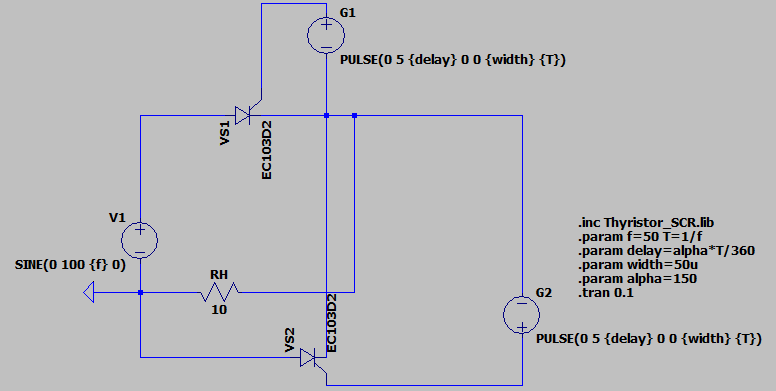
\includegraphics[scale=0.22]{scheme1.png}
        \captionsetup{skip=0pt}
        \caption{Двухполупериодный управляемый выпрямитель с выводом от средней точки}
        \label{fig:scheme1}
    \end{figure}


    \subsection{Регулировочная хар-ка выпрямителя напряжения при активной нагрузке}
    Снимем регулировочную характеристику выпрямителя $U_{\text{вых}}=f\left( \alpha \right)$ при активной нагрузке.
    В таблице представлены средние значения. Угол варьируем в диапазоне $\left[ 30...150 \right]$
    \begin{center}
    \begin{tabular}{ | m{5em} | m{1.5cm}| m{1.5cm} | m{1.5cm} | m{1.5cm} | m{1.5cm} | } 
    \hline
    Угол $\alpha,\left(^\circ\right)$& 30 & 60 & 90 &120 &150 \\ 
    \hline
    $U_{\text{вых}}$, В& 55.1380 & 44.3180 & 29.4850 &14.6660 &3.8619\\ 
    \hline
    \end{tabular}
    \end{center}


    \subsection{Осцилограммы работы выпрямителя напряжения при активной нагрузке}
    Снимем осцилограммы работы выпрямителя при активной нагрузке для различных значений
    угла включения тиристора. Результаты представлены на рис. \ref{fig:a30}--\ref{fig:a150}
    \begin{figure}[H]
        \centering
        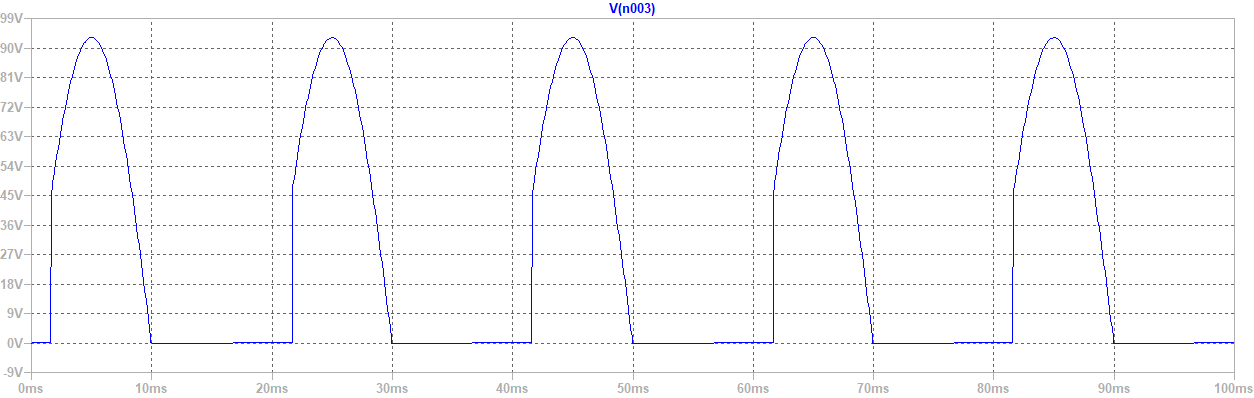
\includegraphics[scale=0.45]{a30.png}
        \captionsetup{skip=0pt}
        \caption{Активная нагрузка, $\alpha=30^{\circ}$}
        \label{fig:a30}
    \end{figure}
    \begin{figure}[H]
        \centering
        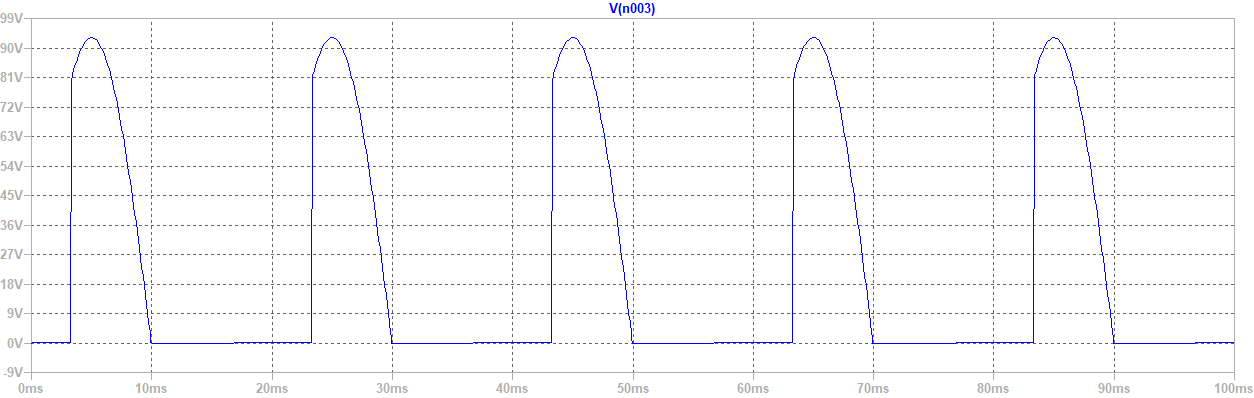
\includegraphics[scale=0.45]{a60.png}
        \captionsetup{skip=0pt}
        \caption{Активная нагрузка, $\alpha=60^{\circ}$}
        \label{fig:a60}
    \end{figure}
    \begin{figure}[H]
        \centering
        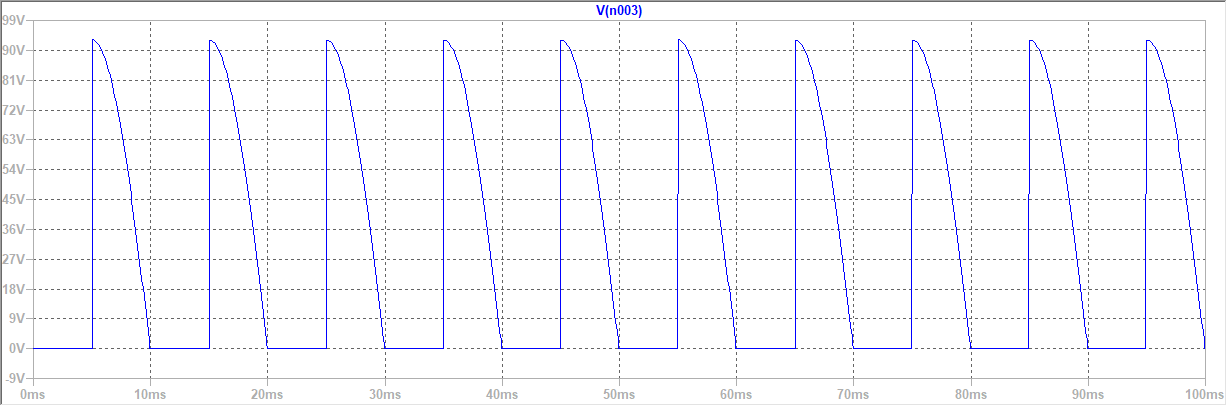
\includegraphics[scale=0.45]{a90.png}
        \captionsetup{skip=0pt}
        \caption{Активная нагрузка, $\alpha=90^{\circ}$}
        \label{fig:a90}
    \end{figure}
    \begin{figure}[H]
        \centering
        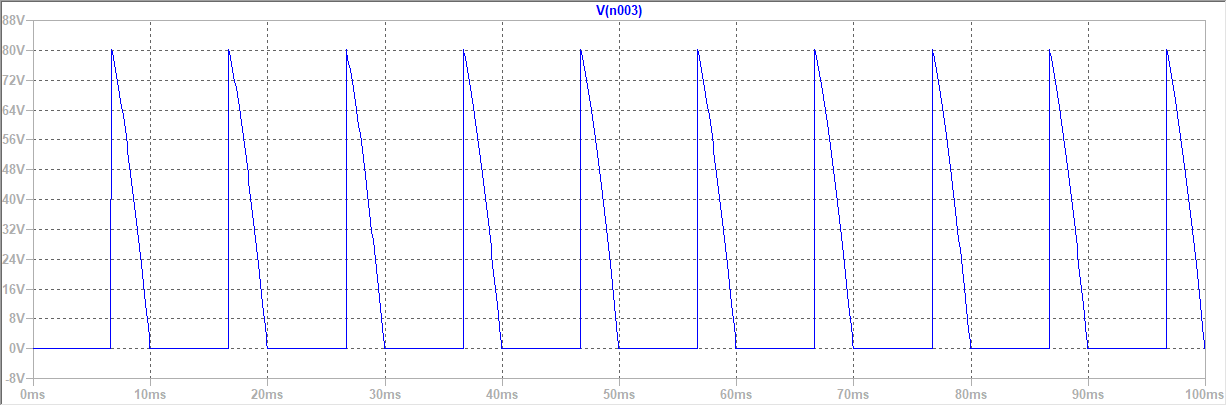
\includegraphics[scale=0.45]{a120.png}
        \captionsetup{skip=0pt}
        \caption{Активная нагрузка, $\alpha=120^{\circ}$}
        \label{fig:a120}
    \end{figure}
    \begin{figure}[H]
        \centering
        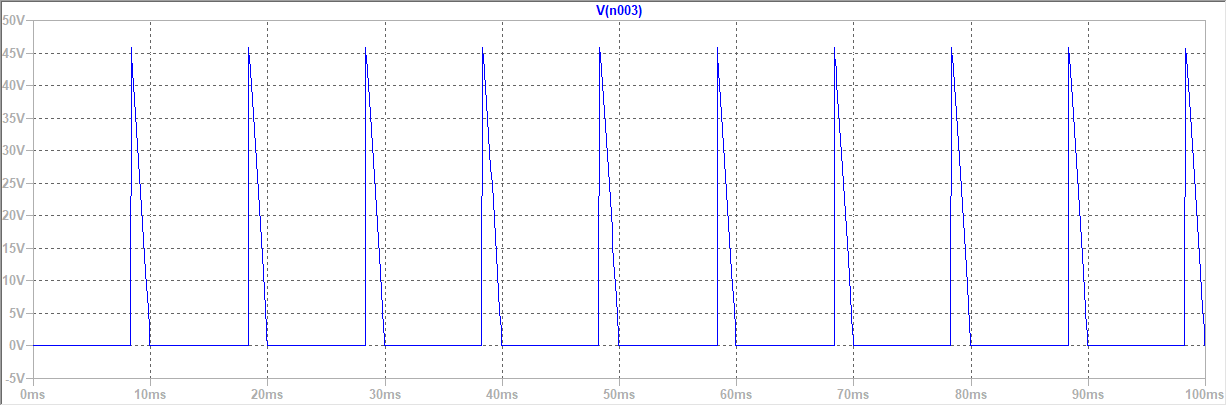
\includegraphics[scale=0.45]{a150.png}
        \captionsetup{skip=0pt}
        \caption{Активная нагрузка, $\alpha=150^{\circ}$}
        \label{fig:a150}
    \end{figure}


    \subsection{Схема выпрямителя напряжения с катушкой индуктивности}
    Добавим в схему перед резистором RH катушку индуктивности L1 с величиной индуктивности 20 мГн
    \begin{figure}[H]
        \centering
        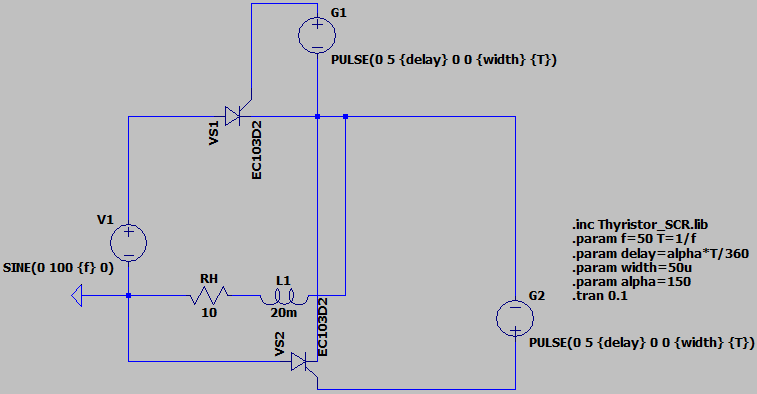
\includegraphics[scale=0.22]{scheme2.png}
        \captionsetup{skip=0pt}
        \caption{Двухполупериодный управляемый выпрямитель с выводом от средней точки}
        \label{fig:scheme2}
    \end{figure}


    \subsection{Осцилограммы работы выпрямителя напряжения при активно-индуктивной нагрузке}
    Снимем осцилограммы работы выпрямителя напряжения при активно-индуктивной нагрузке для различных значений
    угла включения тиристора. Результаты представлены на рис. \ref{fig:a30_L20m}--\ref{fig:a150_L20m}
    \begin{figure}[H]
        \centering
        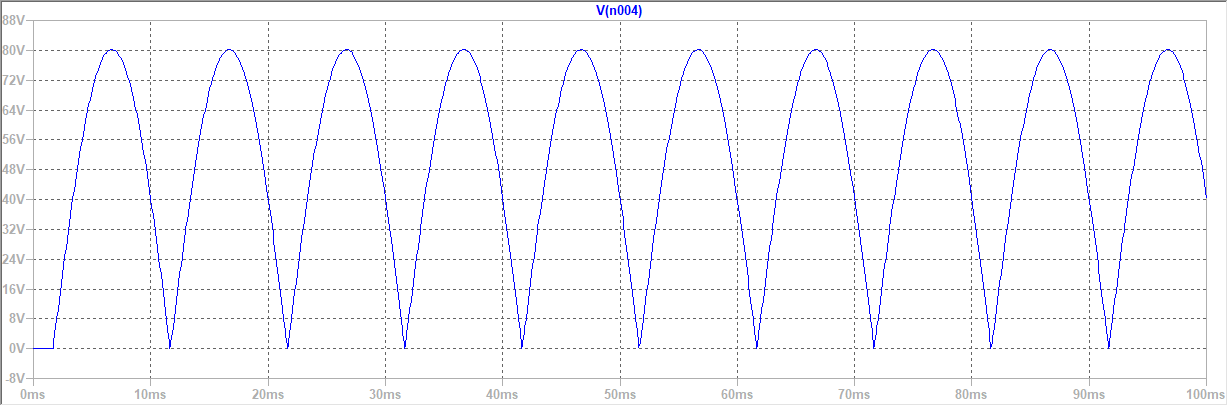
\includegraphics[scale=0.45]{a30_L20m.png}
        \captionsetup{skip=0pt}
        \caption{Активно-индуктивная нагрузка, $\alpha=30^{\circ}$, $L=20$ мГн}
        \label{fig:a30_L20m}
    \end{figure}
    \begin{figure}[H]
        \centering
        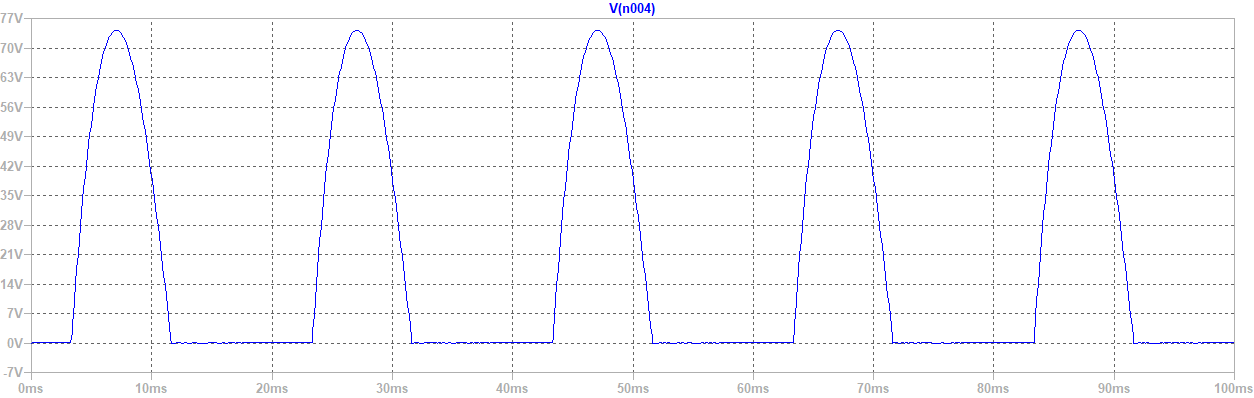
\includegraphics[scale=0.45]{a60_L20m.png}
        \captionsetup{skip=0pt}
        \caption{Активно-индуктивная нагрузка, $\alpha=60^{\circ}$, $L=20$ мГн}
        \label{fig:a60_L20m}
    \end{figure}
    \begin{figure}[H]
        \centering
        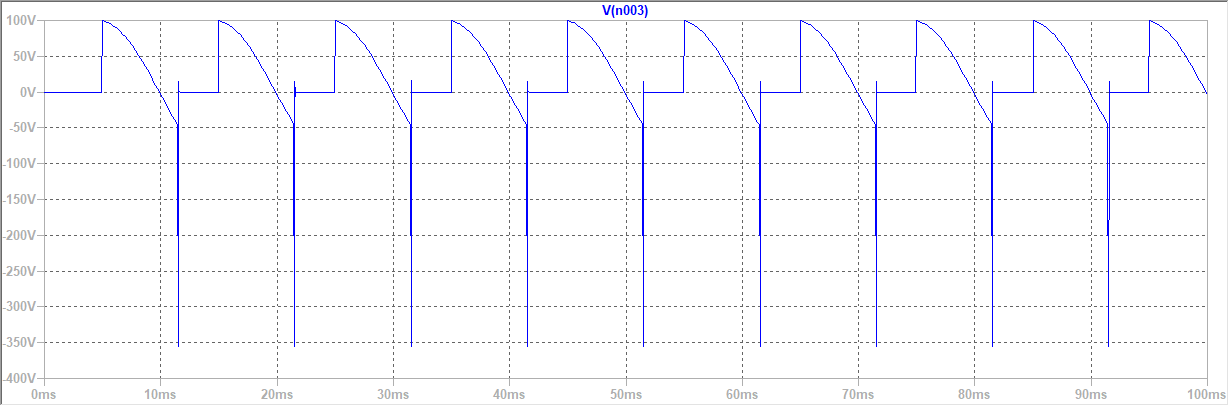
\includegraphics[scale=0.45]{a90_L20m.png}
        \captionsetup{skip=0pt}
        \caption{Активно-индуктивная нагрузка, $\alpha=90^{\circ}$, $L=20$ мГн}
        \label{fig:a90_L20m}
    \end{figure}
    \begin{figure}[H]
        \centering
        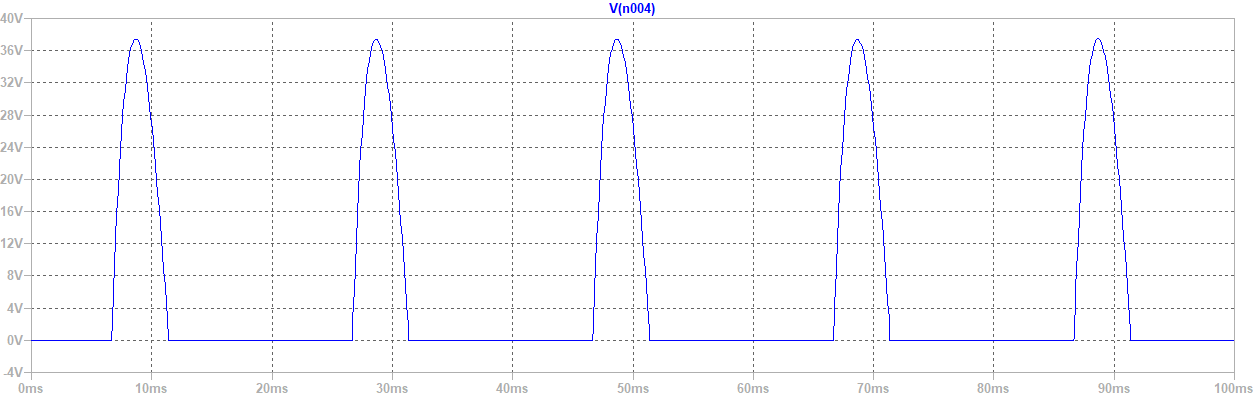
\includegraphics[scale=0.45]{a120_L20m.png}
        \captionsetup{skip=0pt}
        \caption{Активно-индуктивная нагрузка, $\alpha=120^{\circ}$, $L=20$ мГн}
        \label{fig:a120_L20m}
    \end{figure}
    \begin{figure}[H]
        \centering
        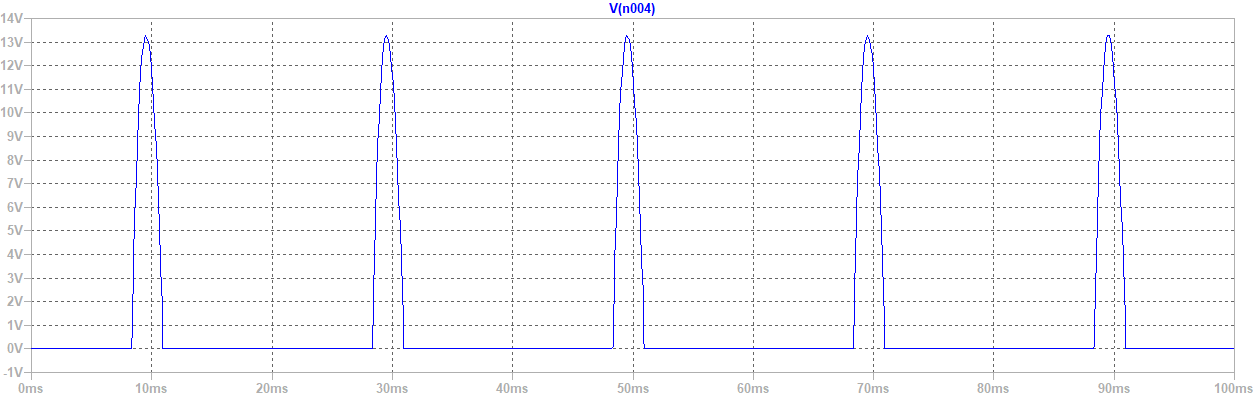
\includegraphics[scale=0.45]{a150_L20m.png}
        \captionsetup{skip=0pt}
        \caption{Активно-индуктивная нагрузка, $\alpha=150^{\circ}$, $L=20$ мГн}
        \label{fig:a150_L20m}
    \end{figure}
    \vfill


    \subsection{Схема выпрямителя напряжения с катушкой индуктивности и диодом}
    Добавим в схему диод D1 параллельно RH и L1. Катод подключим перед катушкой индуктивности,
    анод к земле
    \begin{figure}[H]
        \centering
        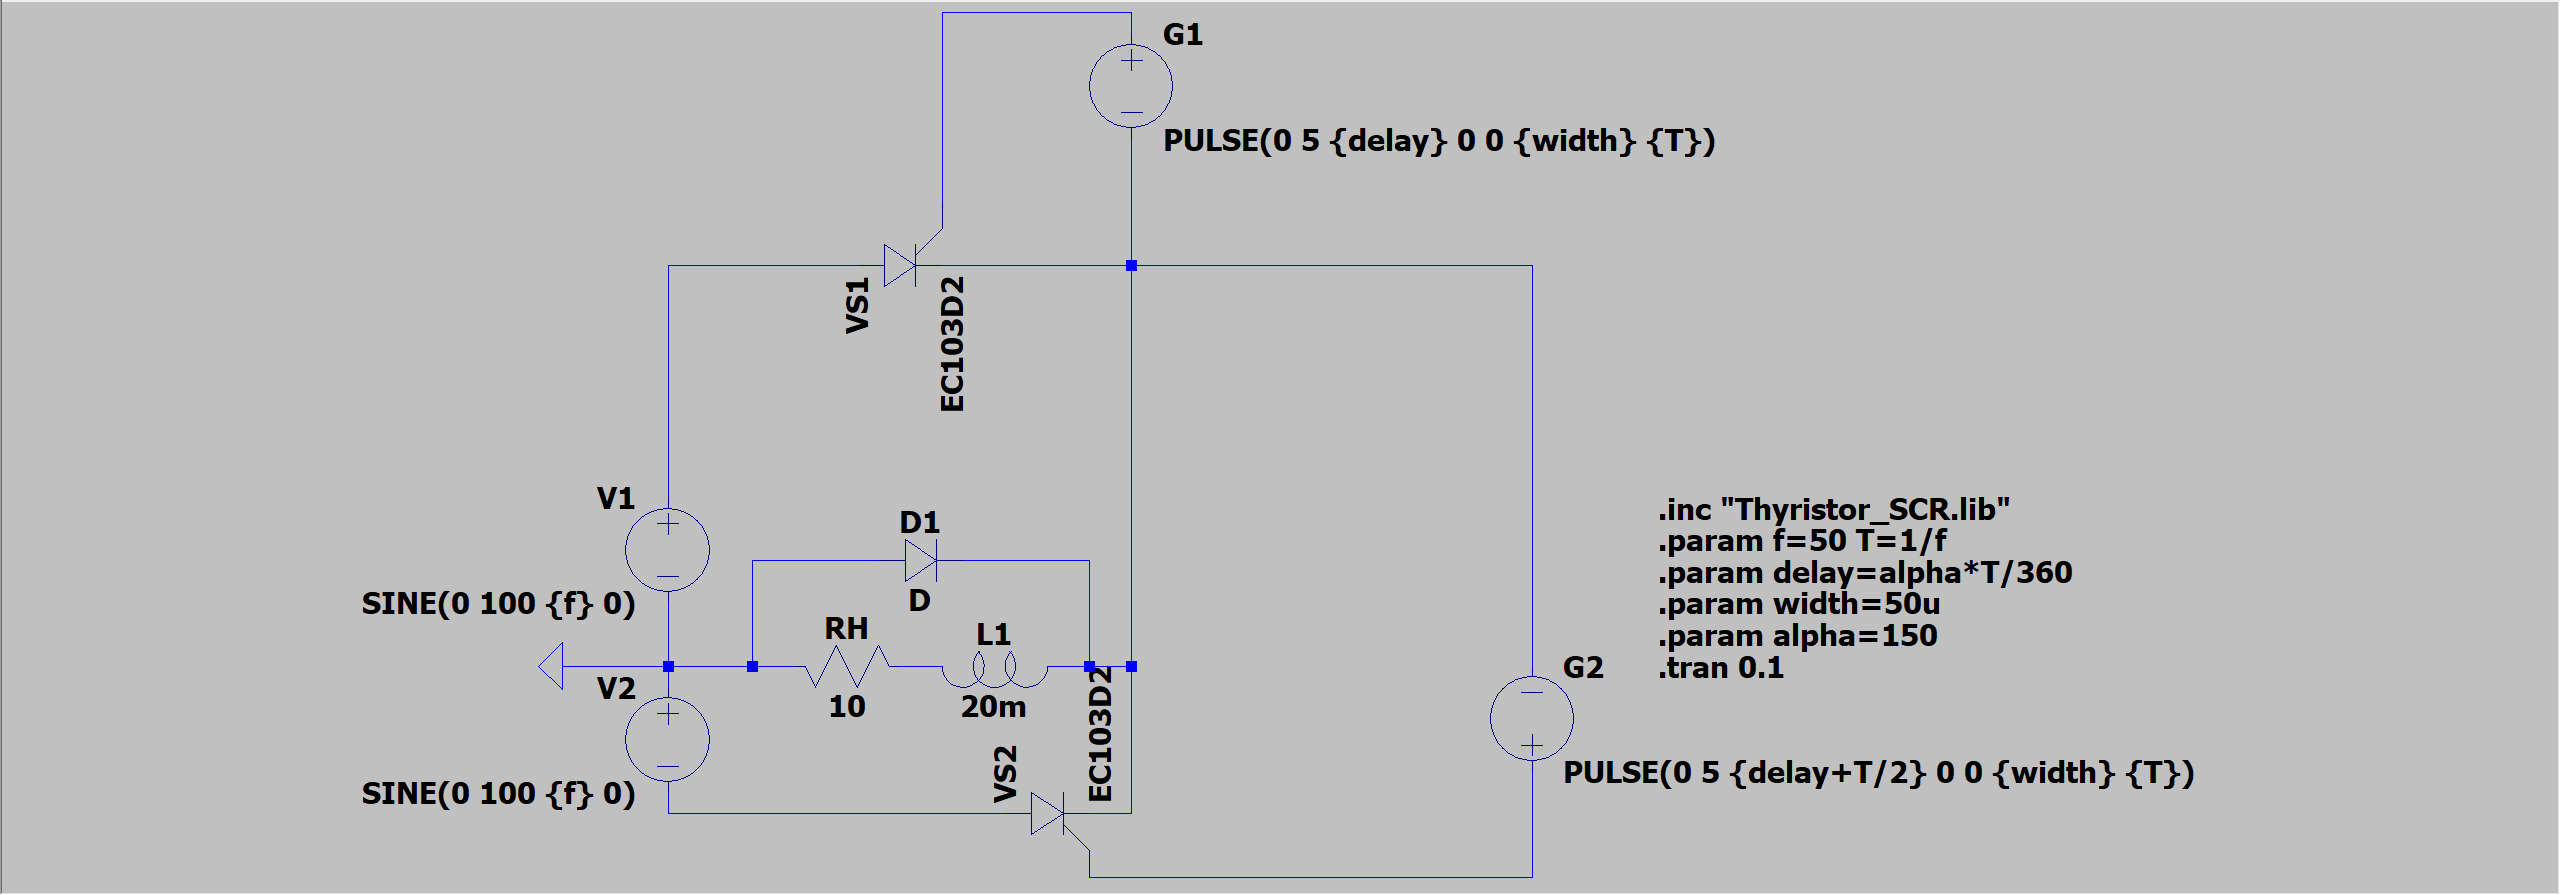
\includegraphics[scale=0.22]{scheme3.png}
        \captionsetup{skip=0pt}
        \caption{Двухполупериодный управляемый выпрямитель с выводом от средней точки}
        \label{fig:scheme3}
    \end{figure}


    \subsection{Осцилограммы работы выпрямителя напряжения при активно-индуктивной нагрузке, шунтированной диодом}
    Снимем осцилограммы работы выпрямителя при активно-индуктивной нагрузке, шунтированной диодом, для различных значений
    угла включения тиристора. Результаты представлены на рис. \ref{fig:a30_L20m_D}--\ref{fig:a150_L20m_D}
    \begin{figure}[H]
        \centering
        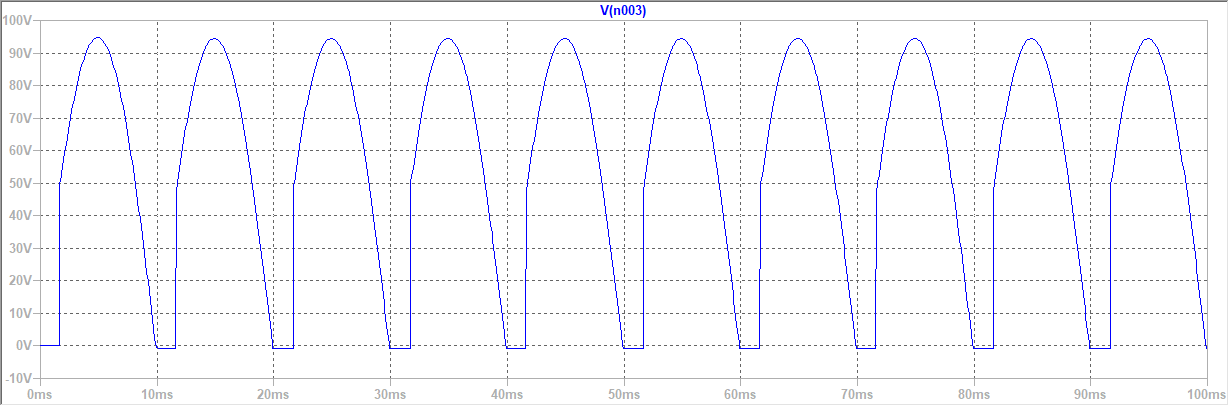
\includegraphics[scale=0.45]{a30_L20m_D.png}
        \captionsetup{skip=0pt}
        \caption{Активно-индуктивная нагрузка с диодом, $\alpha=30^{\circ}$}
        \label{fig:a30_L20m_D}
    \end{figure}
    \begin{figure}[H]
        \centering
        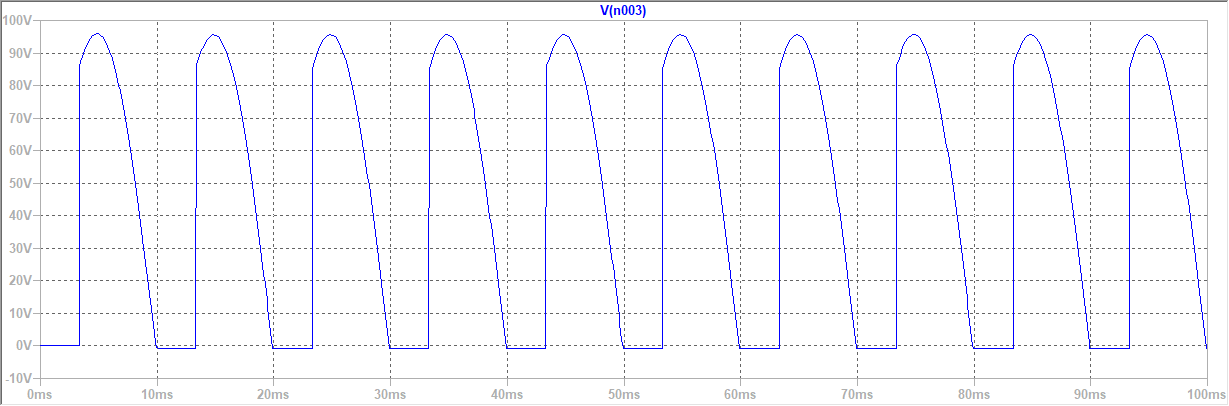
\includegraphics[scale=0.45]{a60_L20m_D.png}
        \captionsetup{skip=0pt}
        \caption{Активно-индуктивная нагрузка с диодом, $\alpha=60^{\circ}$}
        \label{fig:a60_L20m_D}
    \end{figure}
    \begin{figure}[H]
        \centering
        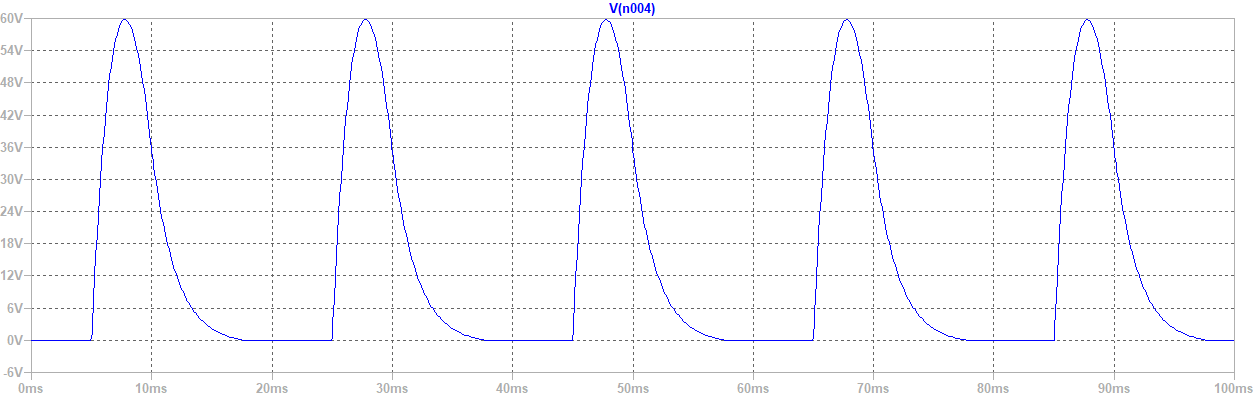
\includegraphics[scale=0.45]{a90_L20m_D.png}
        \captionsetup{skip=0pt}
        \caption{Активно-индуктивная нагрузка с диодом, $\alpha=90^{\circ}$}
        \label{fig:a90_L20m_D}
    \end{figure}
    \begin{figure}[H]
        \centering
        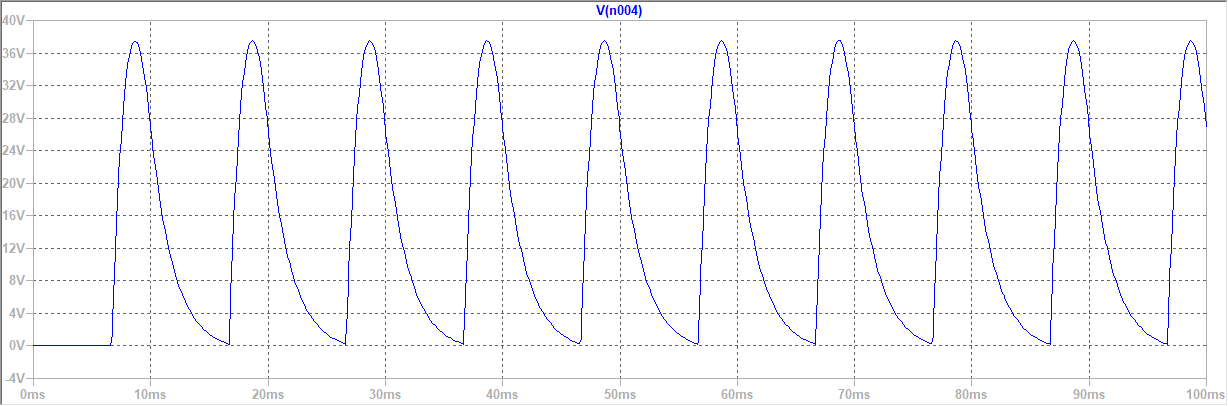
\includegraphics[scale=0.45]{a120_L20m_D.png}
        \captionsetup{skip=0pt}
        \caption{Активно-индуктивная нагрузка с диодом, $\alpha=120^{\circ}$}
        \label{fig:a120_L20m_D}
    \end{figure}
    \begin{figure}[H]
        \centering
        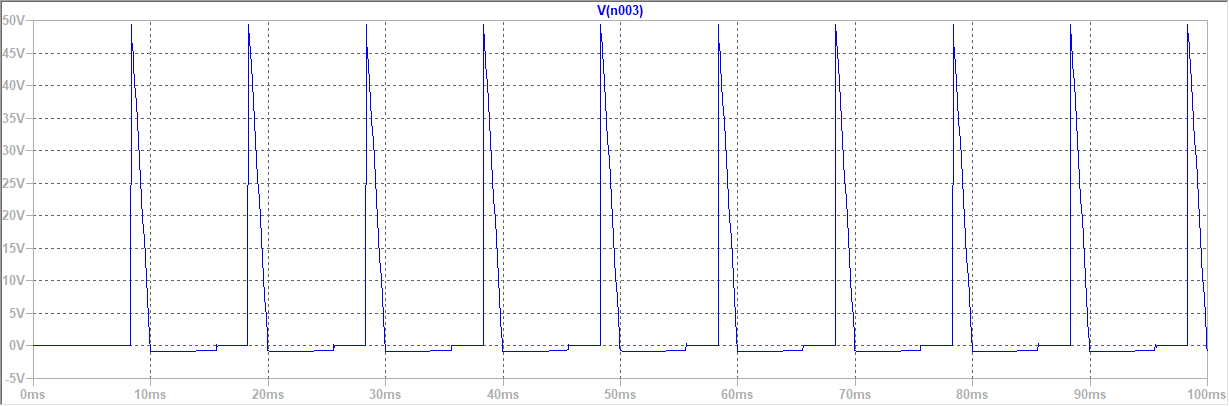
\includegraphics[scale=0.45]{a150_L20m_D.png}
        \captionsetup{skip=0pt}
        \caption{Активно-индуктивная нагрузка с диодом, $\alpha=150^{\circ}$}
        \label{fig:a150_L20m_D}
    \end{figure}
    \vfill


    \section{Задание 2}
    \subsection{Схема регулятора напряжения переменного тока}
    Построим схему регулятора переменного напряжения. Используем симметричный динистор U1 (DIAC)
    и симистор U2 (двунаправленные тиристоры -- триаки)
    \begin{figure}[H]
        \centering
        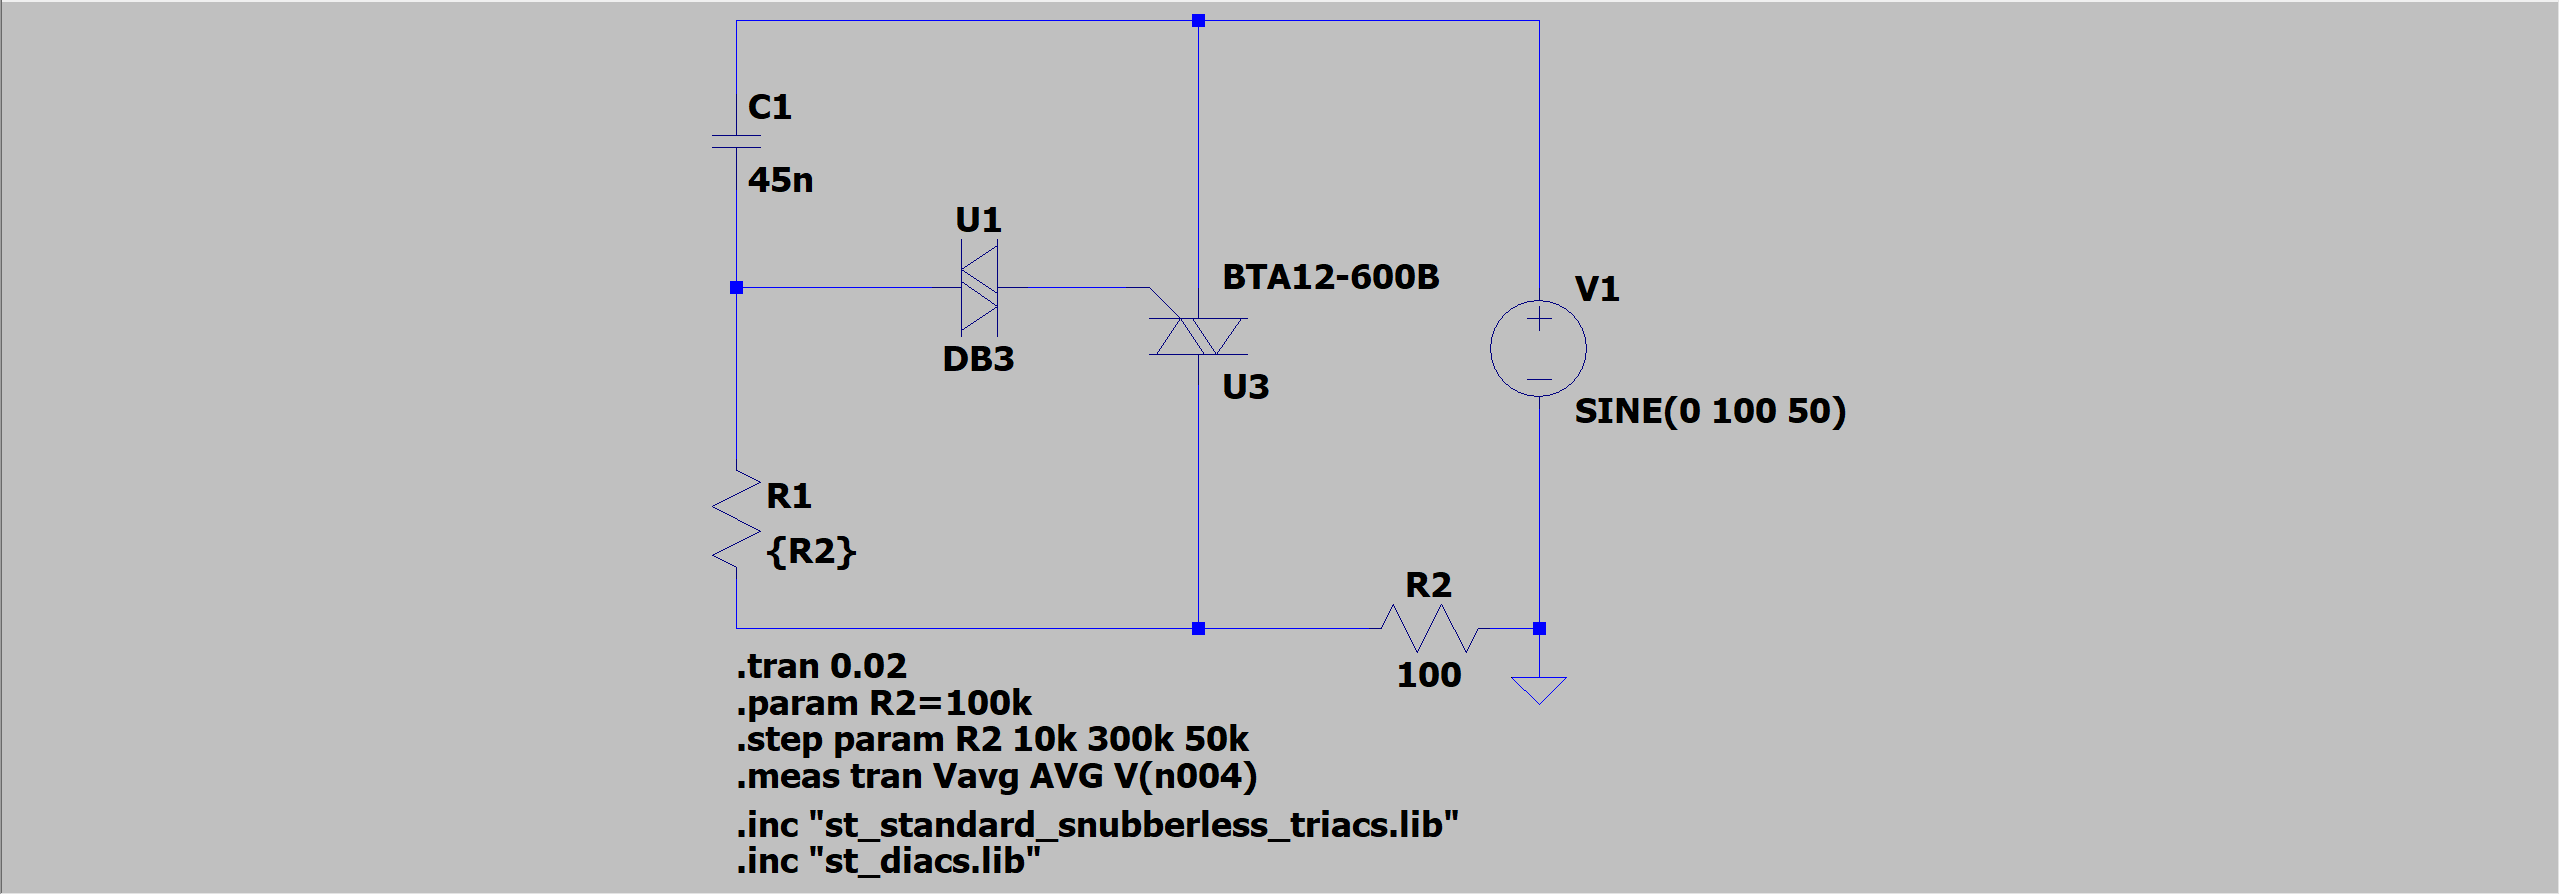
\includegraphics[scale=0.3]{scheme4.png}
        \captionsetup{skip=0pt}
        \caption{Регулятор напряжения переменного тока}
        \label{fig:scheme4}
    \end{figure}


    \subsection{Регулировочная характеристика регулятора напряжения при активной нагрузке}
    Снимем регулировочную характеристику регулятора напряжения $U_{\text{вых}}=f\left( R \right)$
    при активной нагрузке. В таблице представлены средние значения. Сопротивление R1 варьируем от $10\cdot10^3$ до $300\cdot10^3$
    с шагом $50\cdot10^3$
    \begin{center}
        \begin{tabular}{ | m{4em} | m{1.5cm}| m{1.5cm} | m{1.5cm} | m{1.5cm} | m{1.5cm} | m{1.5cm} | m{1.5cm} | } 
        \hline
        $R,$ Ом& $10\cdot10^3$ & $60\cdot10^3$ & $110\cdot10^3$ &$160\cdot10^3$ &$210\cdot10^3$ &$260\cdot10^3$ &$300\cdot10^3$ \\ 
        \hline
        $U_{\text{вых}}$, В& 0.0263 & 0.3374 & 1.2721 &2.731 &4.6158 &7.8872 &3.2499\\ 
        \hline
    \end{tabular}
    \end{center}


    \subsection{Осцилограммы работы регулятора напряжения при активной нагрузке}
    Снимем осцилограммы работы регулятора при активной нагрузке
    для различных значений сопротивления R1. Результаты представлены на рис. \ref{fig:R2-all}-\ref{fig:R2-300k}
    \begin{figure}[H]
        \centering
        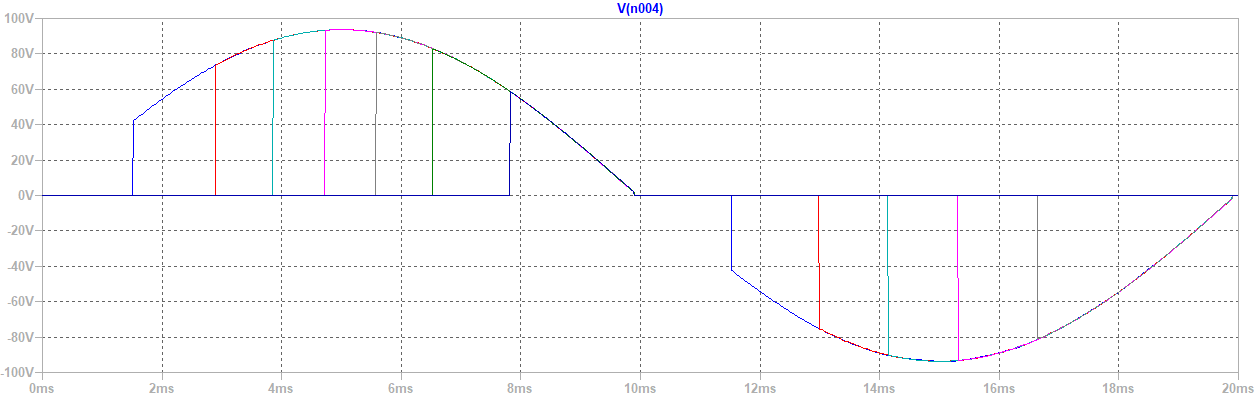
\includegraphics[scale=0.45]{R2-all.png}
        \captionsetup{skip=0pt}
        \caption{Активная нагрузка, $R\in10^3\cdot\left[ 10...300 \right]$ Ом, шаг $50\cdot10^3$ Ом}
        \label{fig:R2-all}
    \end{figure}
    \begin{figure}[H]
        \centering
        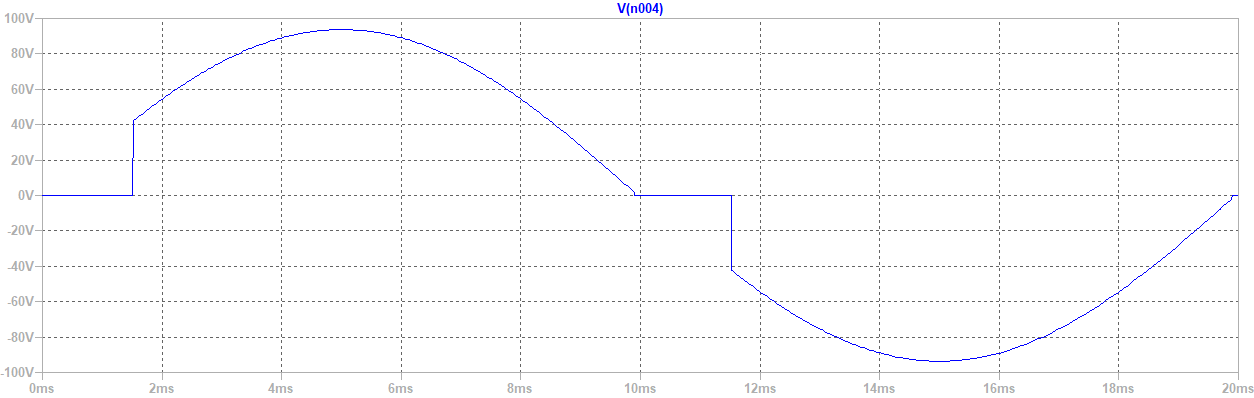
\includegraphics[scale=0.45]{R2-10k.png}
        \captionsetup{skip=0pt}
        \caption{Активная нагрузка, $R=10\cdot10^3$ Ом}
        \label{fig:R2-10k}
    \end{figure}
    \begin{figure}[H]
        \centering
        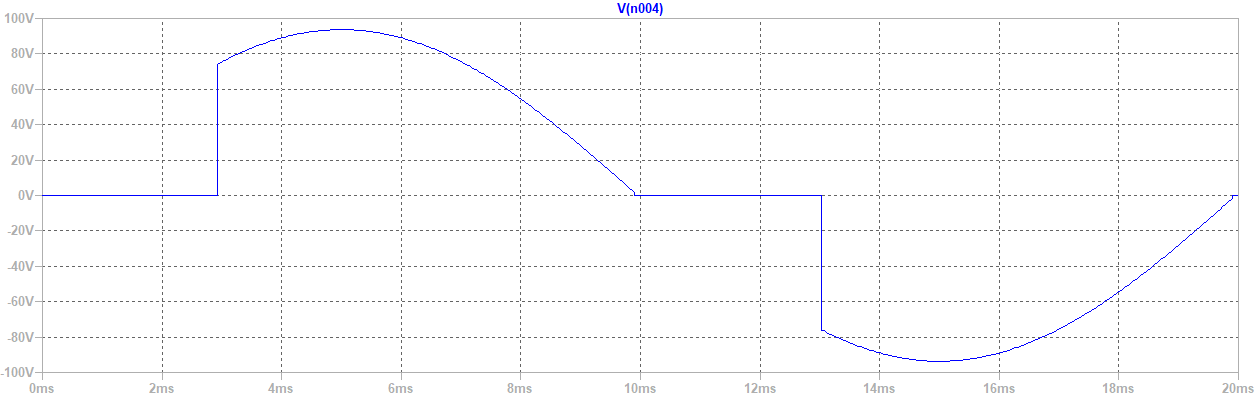
\includegraphics[scale=0.45]{R2-60k.png}
        \captionsetup{skip=0pt}
        \caption{Активная нагрузка, $R=60\cdot10^3$ Ом}
        \label{fig:R2-60k}
    \end{figure}
    \begin{figure}[H]
        \centering
        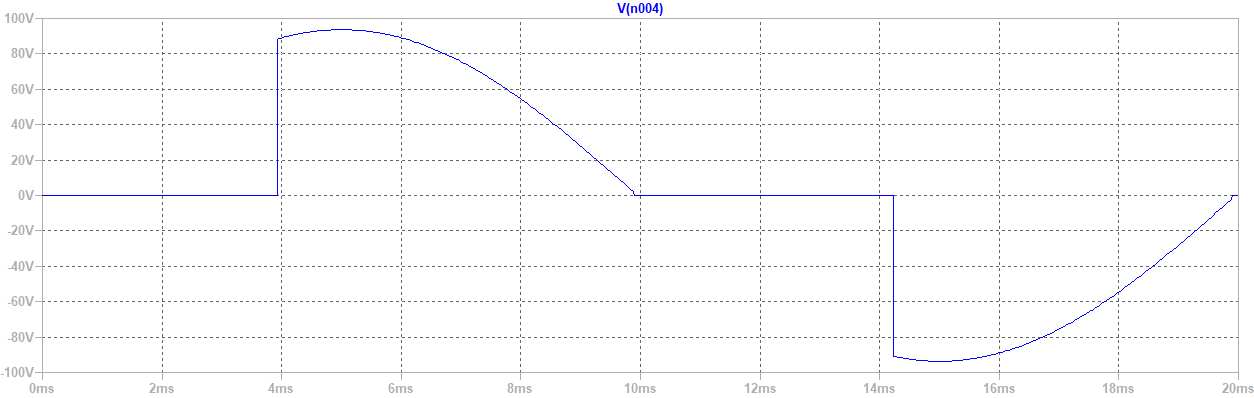
\includegraphics[scale=0.45]{R2-110k.png}
        \captionsetup{skip=0pt}
        \caption{Активная нагрузка, $R=110\cdot10^3$ Ом}
        \label{fig:R2-110k}
    \end{figure}
    \begin{figure}[H]
        \centering
        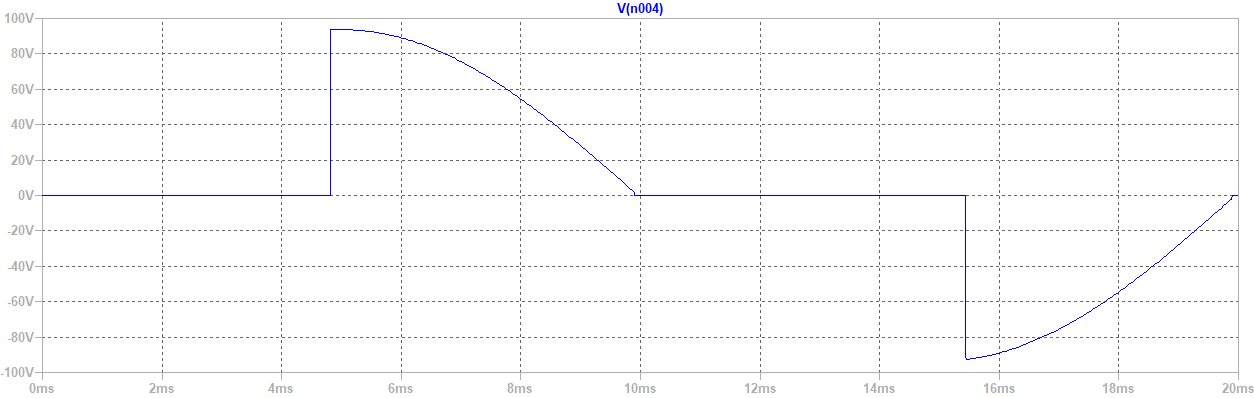
\includegraphics[scale=0.45]{R2-160k.png}
        \captionsetup{skip=0pt}
        \caption{Активная нагрузка, $R=160\cdot10^3$ Ом}
        \label{fig:R2-160k}
    \end{figure}
    \begin{figure}[H]
        \centering
        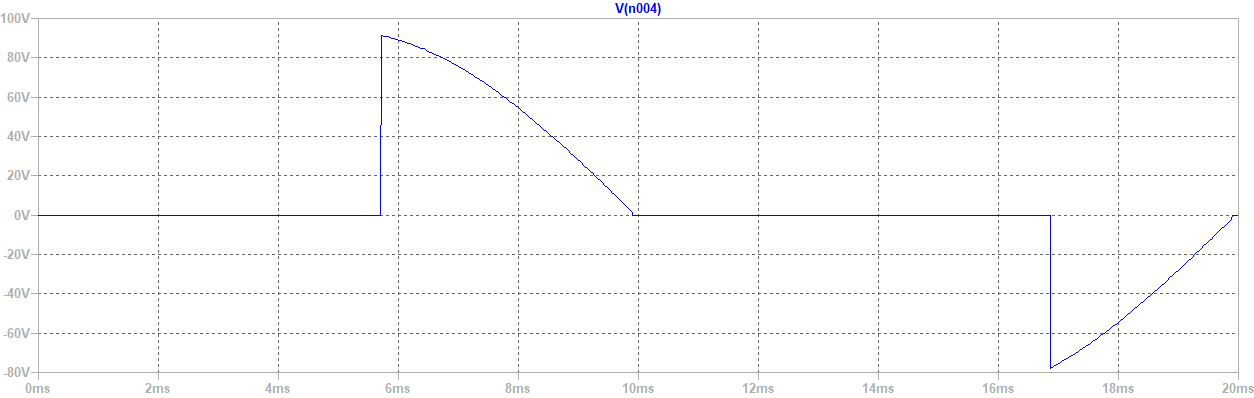
\includegraphics[scale=0.45]{R2-210k.png}
        \captionsetup{skip=0pt}
        \caption{Активная нагрузка, $R=210\cdot10^3$ Ом}
        \label{fig:R2-210k}
    \end{figure}
    \begin{figure}[H]
        \centering
        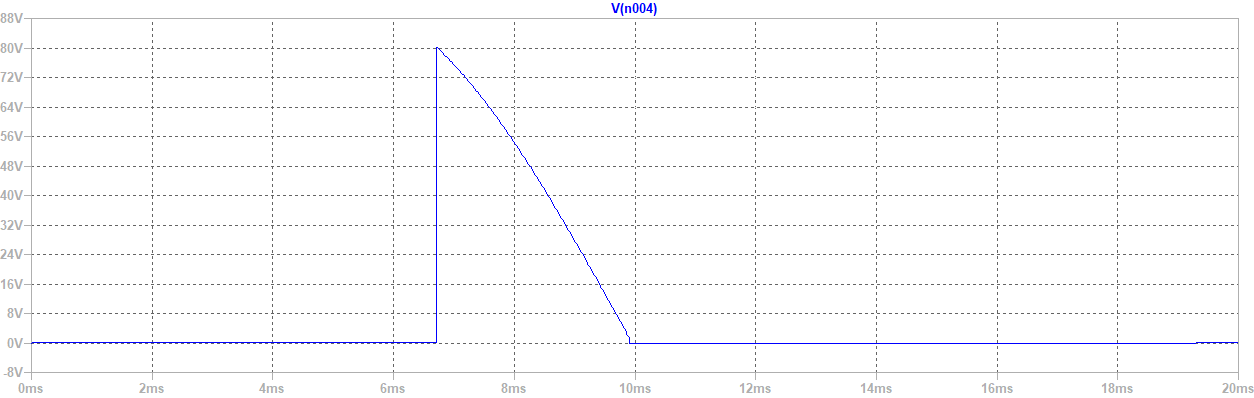
\includegraphics[scale=0.45]{R2-260k.png}
        \captionsetup{skip=0pt}
        \caption{Активная нагрузка, $R=260\cdot10^3$ Ом}
        \label{fig:R2-260k}
    \end{figure}
    \begin{figure}[H]
        \centering
        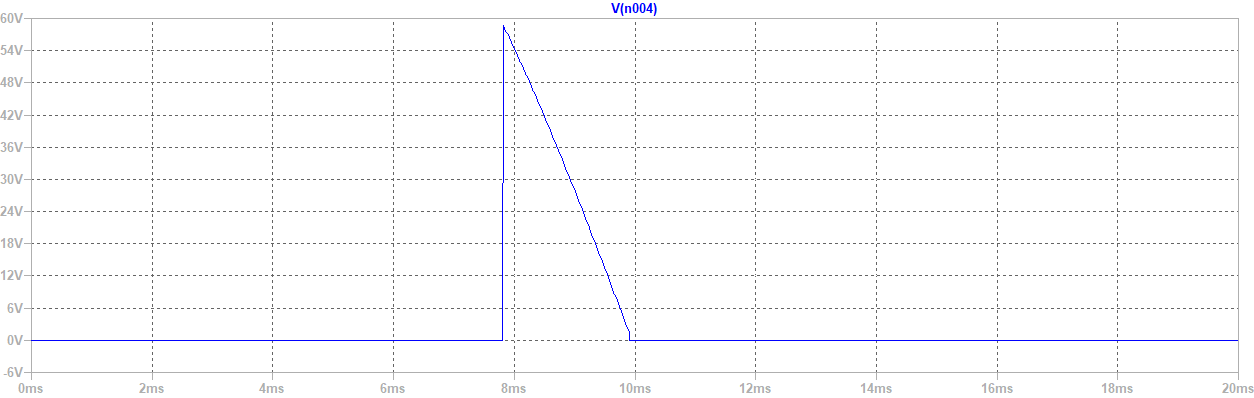
\includegraphics[scale=0.45]{R2-300k.png}
        \captionsetup{skip=0pt}
        \caption{Активная нагрузка, $R=300\cdot10^3$ Ом}
        \label{fig:R2-300k}
    \end{figure}
    \vfill


    \subsection{Схема регулятора напряжения с катушкой индуктивности}
    Добавим в схему перед R2 катушку индуктивности с величиной индуктивности 20 мГн
    \begin{figure}[H]
        \centering
        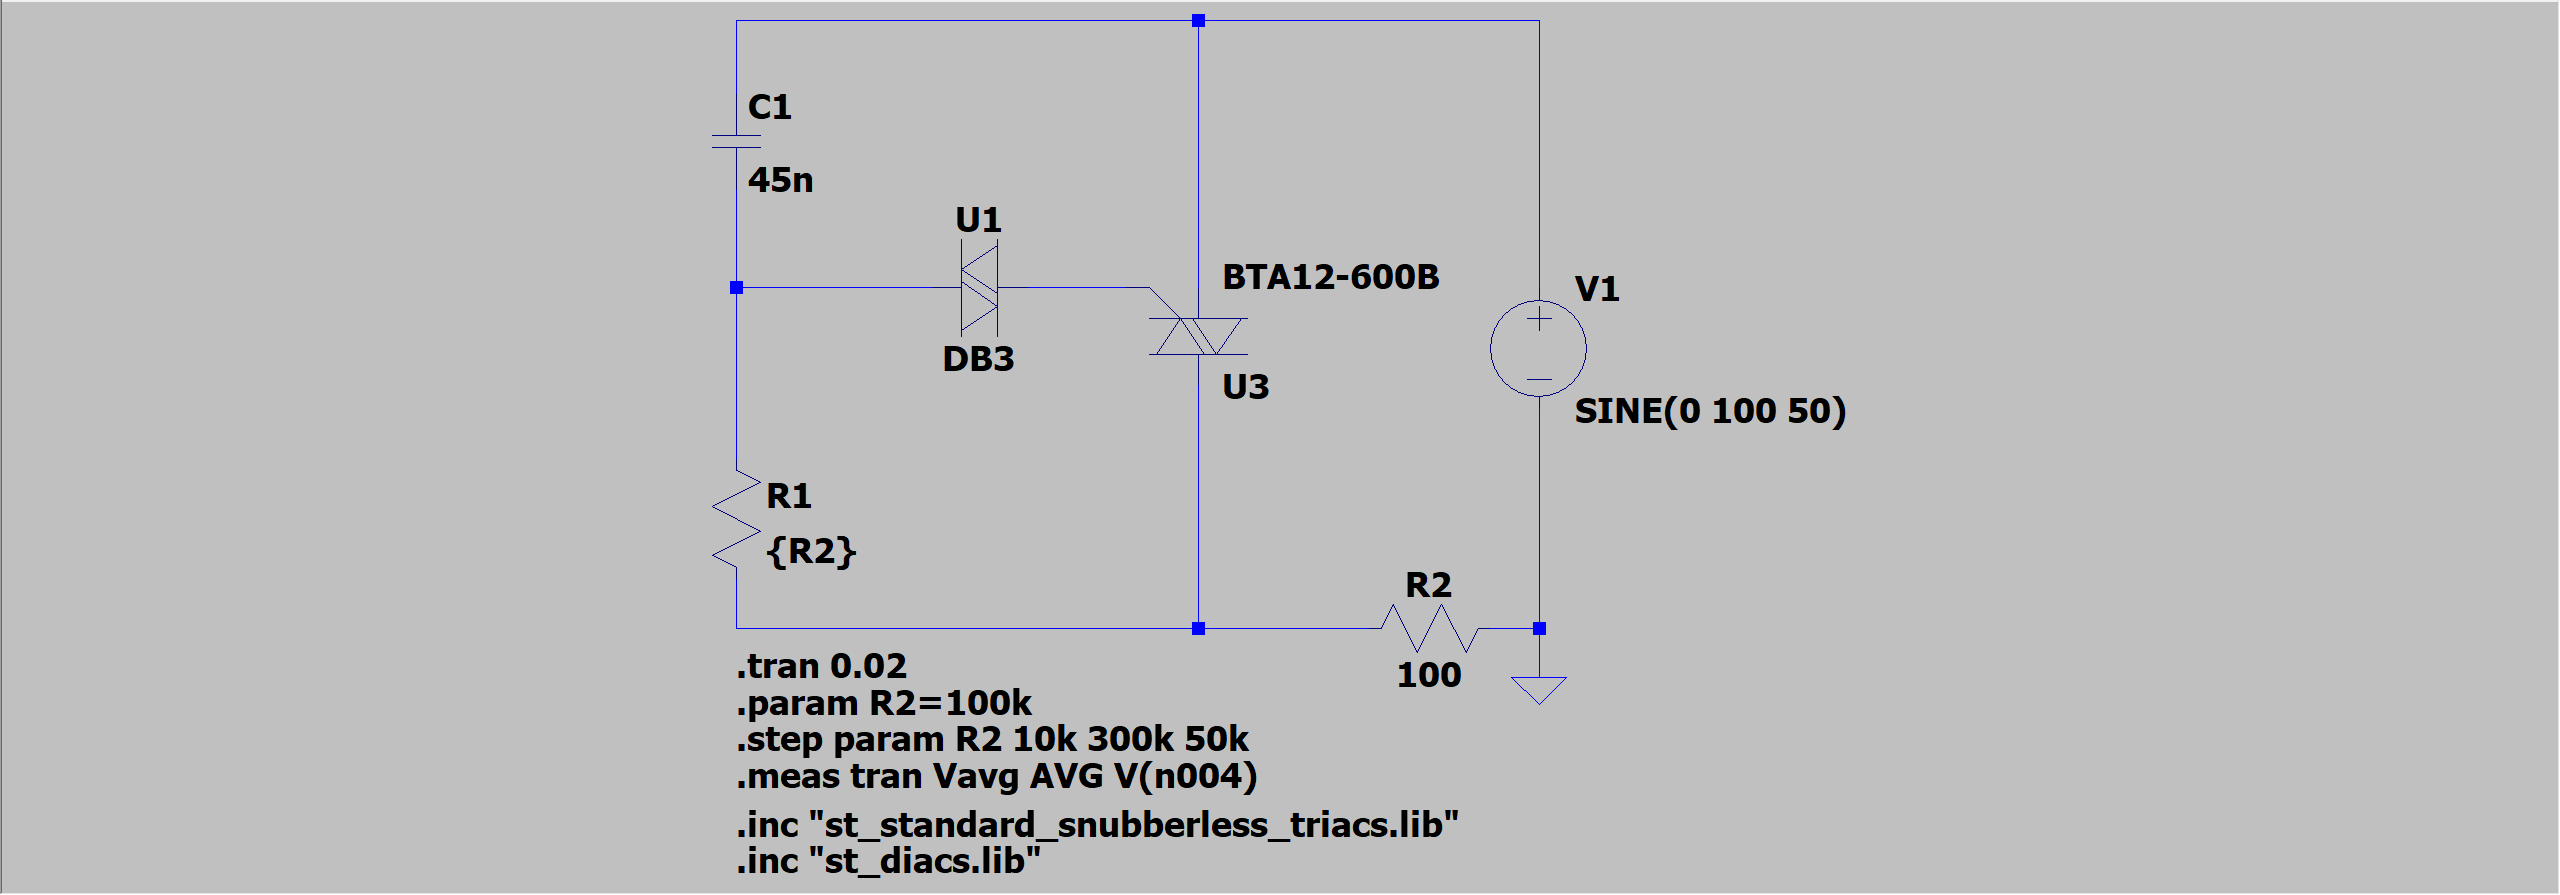
\includegraphics[scale=0.3]{scheme5.png}
        \captionsetup{skip=0pt}
        \caption{Регулятор напряжения переменного тока}
        \label{fig:scheme5}
    \end{figure}


    \subsection{Осцилограммы работы регулятора напряжения при активно-индуктивной нагрузке}
    Снимем осцилограммы работы регулятора при активно-индуктивной нагрузке
    для различных значений сопротивления R1. Рез-ы представлены на рис. \ref{fig:R2-all_L20m}-\ref{fig:R2-300k_L20m}
    \begin{figure}[H]
        \centering
        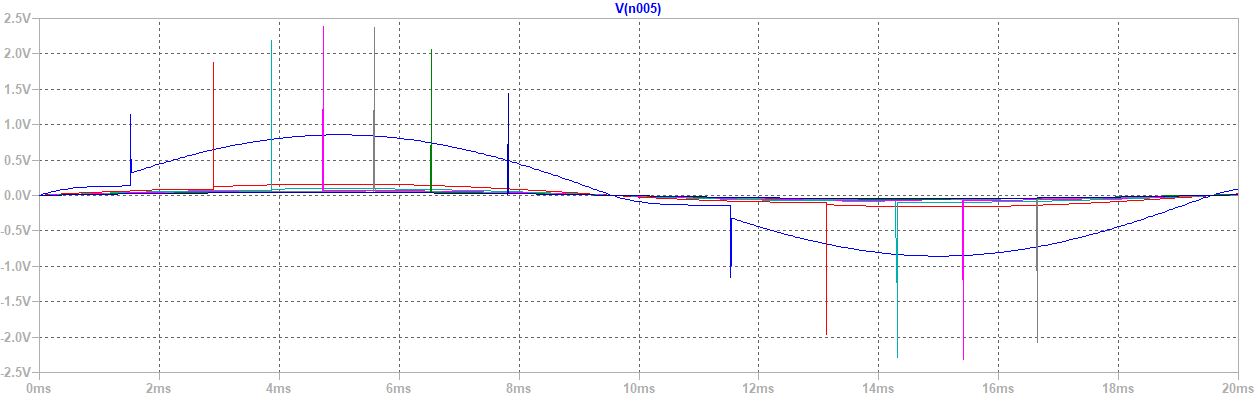
\includegraphics[scale=0.45]{R2-all_L20m.png}
        \captionsetup{skip=0pt}
        \caption{Активно-индукт. нагр., $R\in10^3\cdot\left[ 10...300 \right]$ Ом, шаг $50\cdot10^3$ Ом, $L=20$ мГн}
        \label{fig:R2-all_L20m}
    \end{figure}
    \begin{figure}[H]
        \centering
        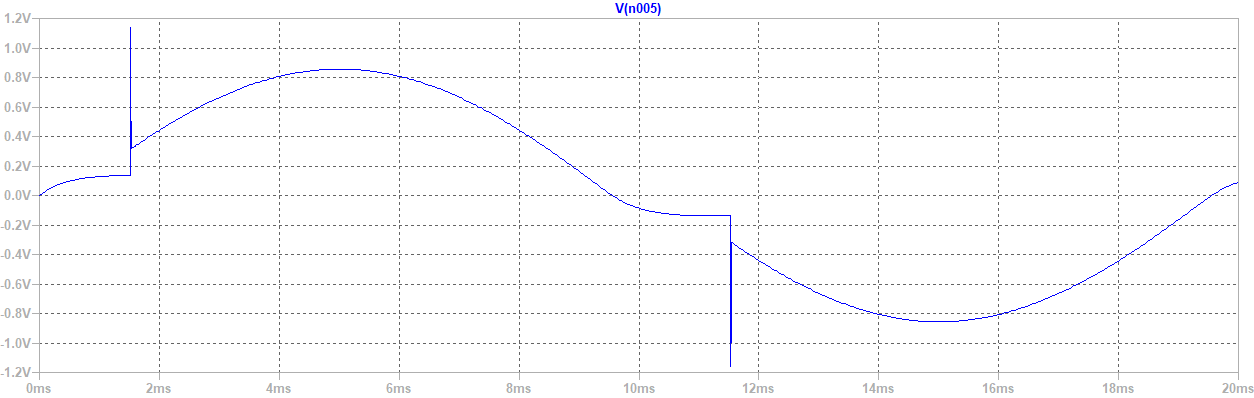
\includegraphics[scale=0.45]{R2-10k_L20m.png}
        \captionsetup{skip=0pt}
        \caption{Активно-индуктивная нагрузка, $R=10\cdot10^3$ Ом, $L=20$ мГн}
        \label{fig:R2-10k_L20m}
    \end{figure}
    \begin{figure}[H]
        \centering
        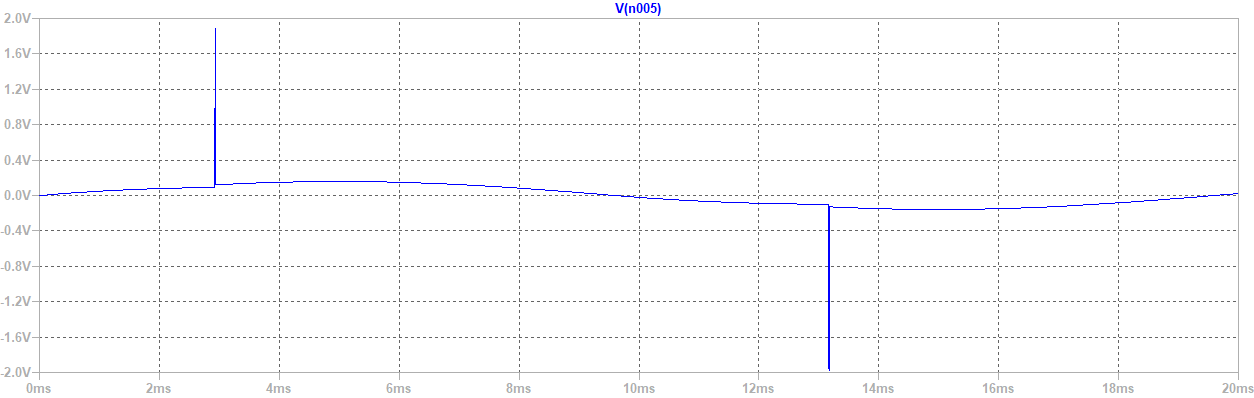
\includegraphics[scale=0.45]{R2-60k_L20m.png}
        \captionsetup{skip=0pt}
        \caption{Активно-индуктивная нагрузка, $R=60\cdot10^3$ Ом, $L=20$ мГн}
        \label{fig:R2-60k_L20m}
    \end{figure}
    \begin{figure}[H]
        \centering
        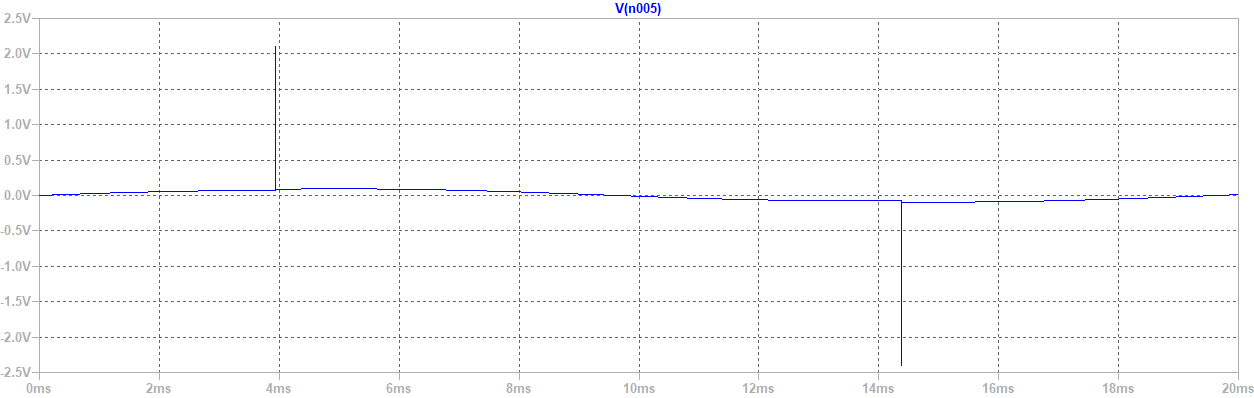
\includegraphics[scale=0.45]{R2-110k_L20m.png}
        \captionsetup{skip=0pt}
        \caption{Активно-индуктивная нагрузка, $R=110\cdot10^3$ Ом, $L=20$ мГн}
        \label{fig:R2-110k_L20m}
    \end{figure}
    \begin{figure}[H]
        \centering
        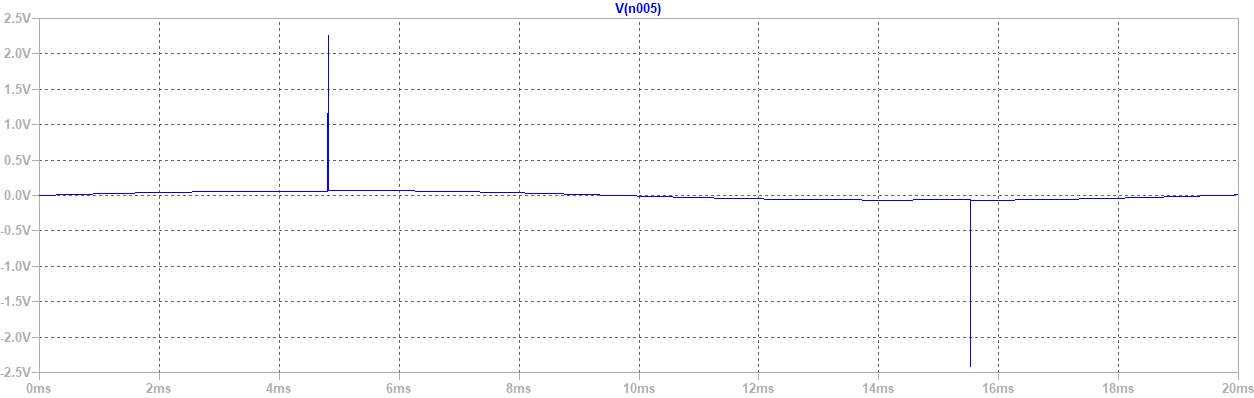
\includegraphics[scale=0.45]{R2-160k_L20m.png}
        \captionsetup{skip=0pt}
        \caption{Активно-индуктивная нагрузка, $R=160\cdot10^3$ Ом, $L=20$ мГн}
        \label{fig:R2-160k_L20m}
    \end{figure}
    \begin{figure}[H]
        \centering
        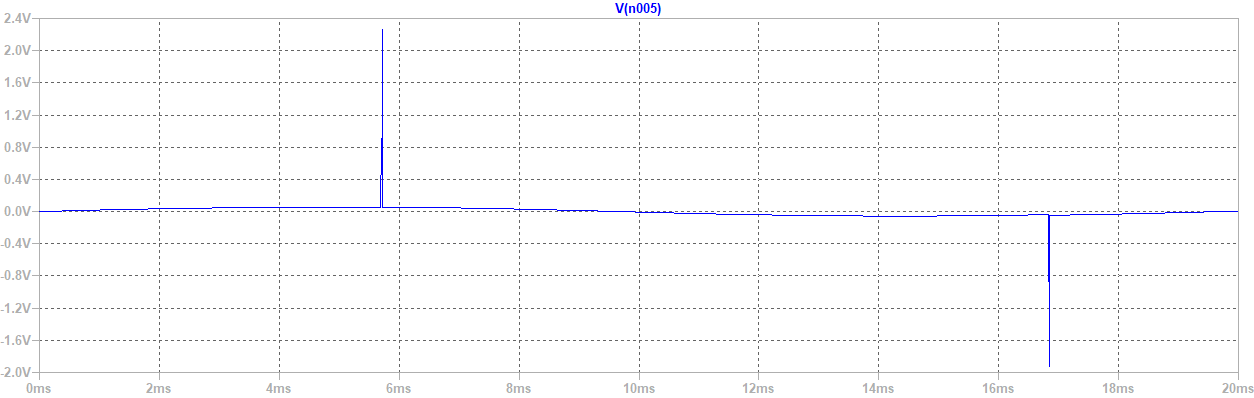
\includegraphics[scale=0.45]{R2-210k_L20m.png}
        \captionsetup{skip=0pt}
        \caption{Активно-индуктивная нагрузка, $R=210\cdot10^3$ Ом, $L=20$ мГн}
        \label{fig:R2-210k_L20m}
    \end{figure}
    \begin{figure}[H]
        \centering
        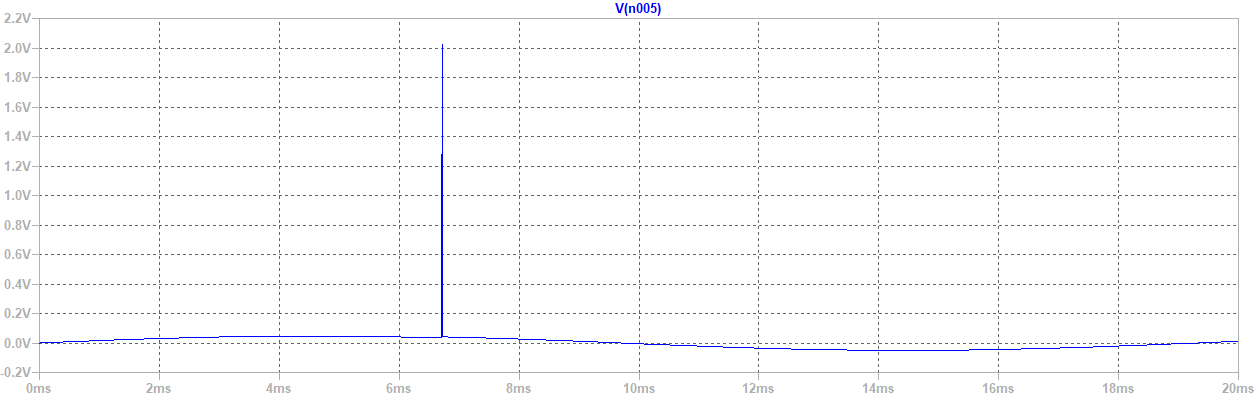
\includegraphics[scale=0.45]{R2-260k_L20m.png}
        \captionsetup{skip=0pt}
        \caption{Активно-индуктивная нагрузка, $R=260\cdot10^3$ Ом, $L=20$ мГн}
        \label{fig:R2-260k_L20m}
    \end{figure}
    \begin{figure}[H]
        \centering
        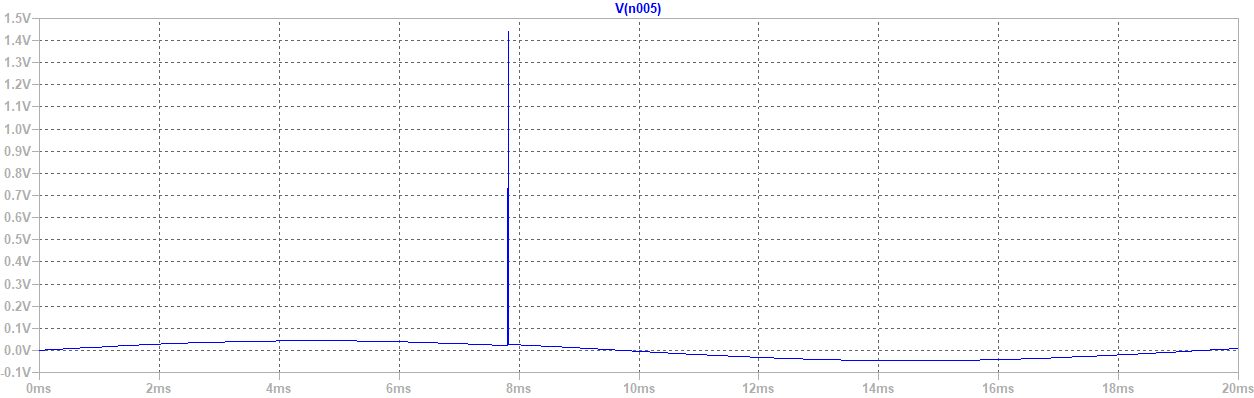
\includegraphics[scale=0.45]{R2-300k_L20m.png}
        \captionsetup{skip=0pt}
        \caption{Активно-индуктивная нагрузка, $R=300\cdot10^3$ Ом, $L=20$ мГн}
        \label{fig:R2-300k_L20m}
    \end{figure}
    \noindent Наблюдаем явление самоиндукции. В подобные схемы катушки индуктивности ставить не нужно.


    \subsection{Схема регулятора напряжения с конденсатором}
    Уберем из схемы катушку индуктивности L1 и добавим конденсатор C2 с емкостью 10 мкФ
    \begin{figure}[H]
        \centering
        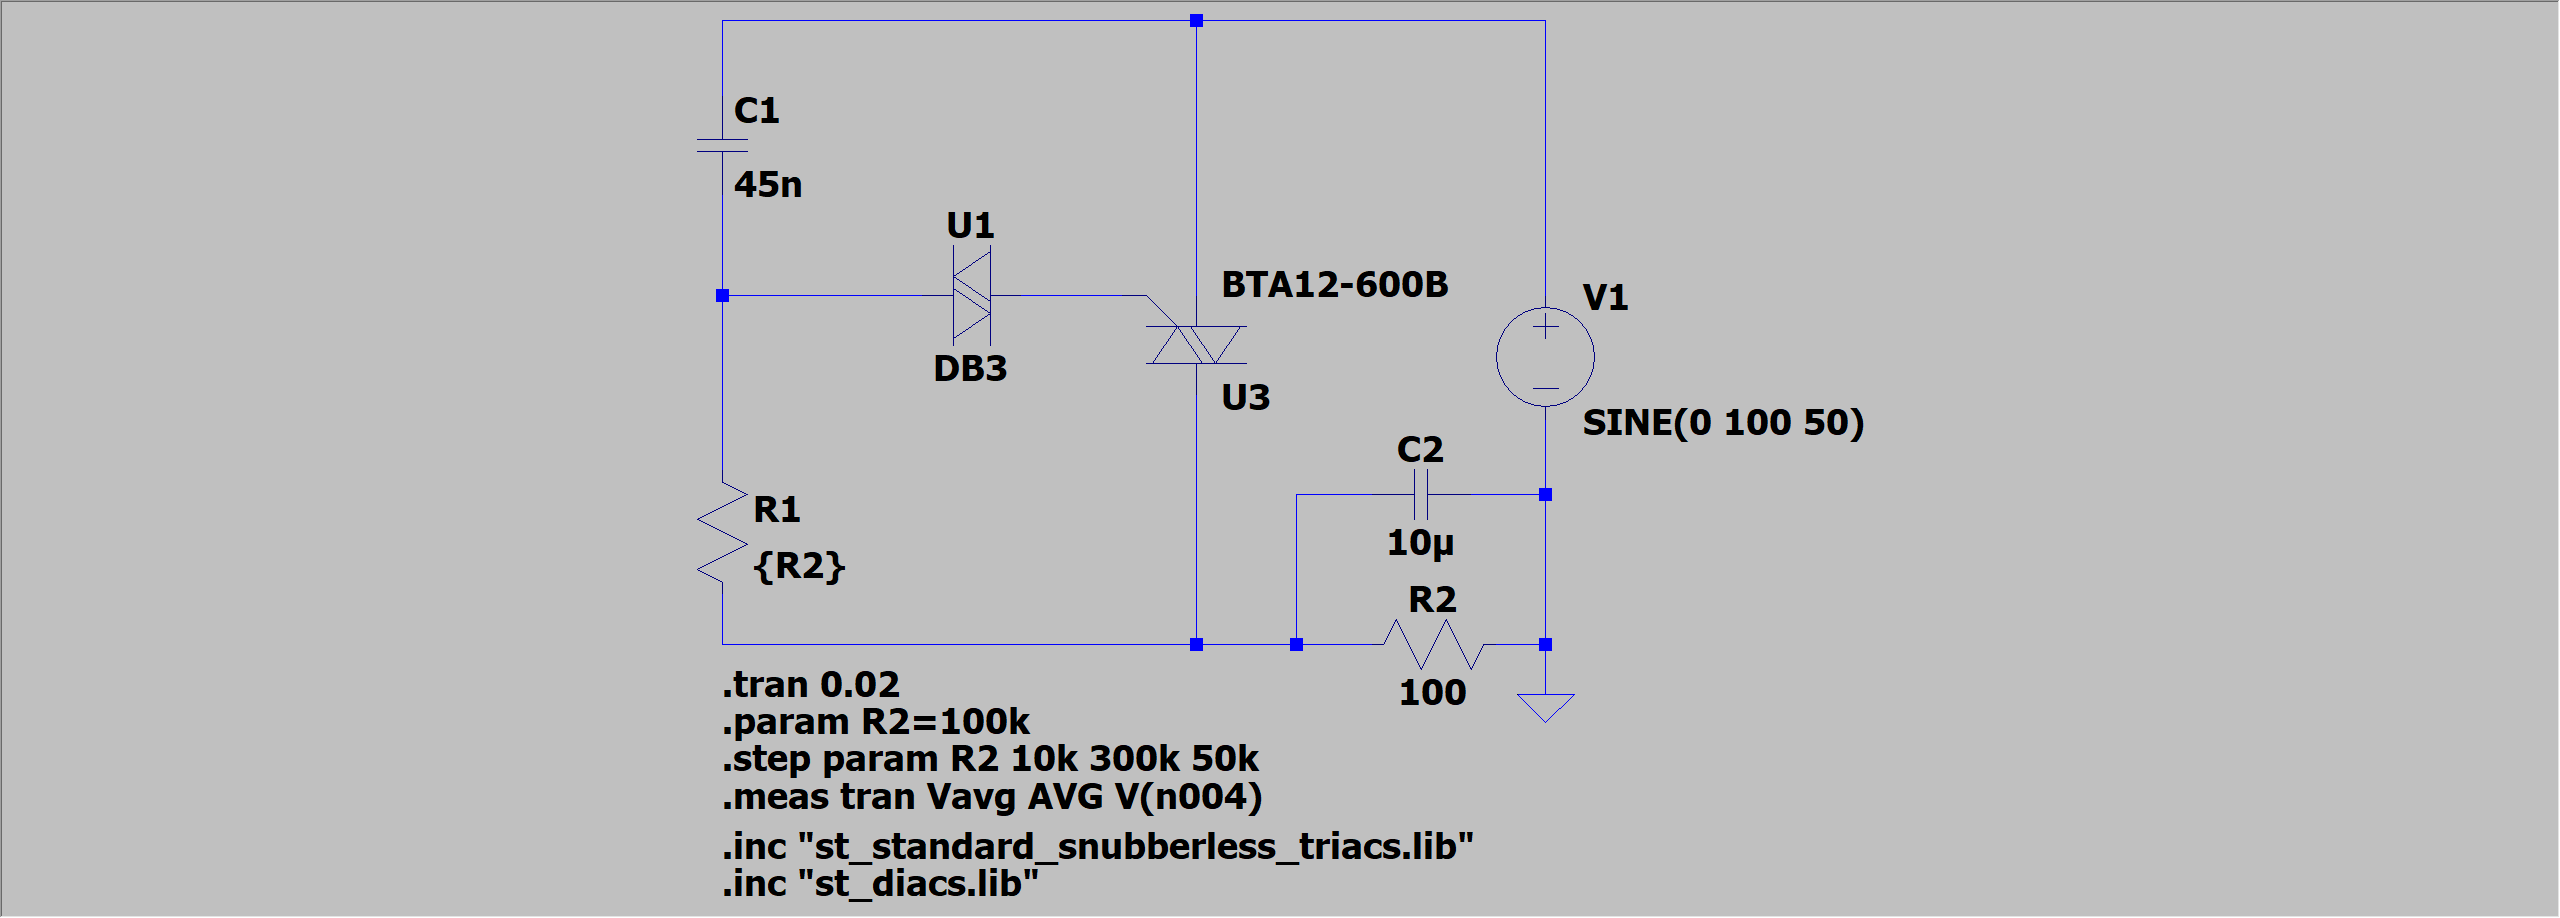
\includegraphics[scale=0.3]{scheme6.png}
        \captionsetup{skip=0pt}
        \caption{Регулятор напряжения переменного тока}
        \label{fig:scheme6}
    \end{figure}


    \subsection{Осцилограммы работы регулятора напряжения при активно-емкостной нагрузке}
    Снимем осцилограммы работы регулятора при активно-емкостной нагрузке 
    для различных значений сопротивления R1. Результаты представлены на рис. \ref{fig:R2-all_C10u}--\ref{fig:R2-300k_C10u}
    \begin{figure}[H]
        \centering
        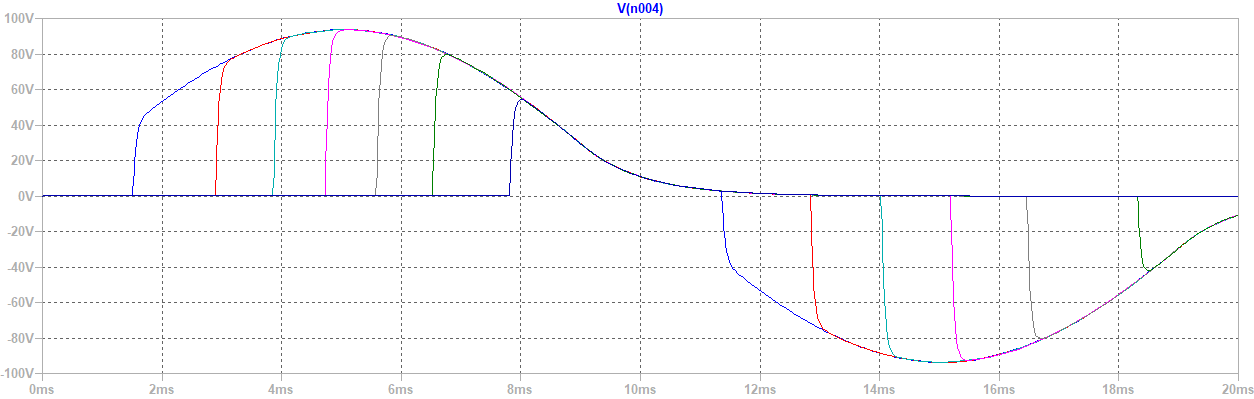
\includegraphics[scale=0.45]{R2-all_C10u.png}
        \captionsetup{skip=0pt}
        \caption{Активно-емкостная нагрузка, $R\in10^3\cdot\left[ 10...300 \right]$ Ом, шаг $50\cdot10^3$ Ом, $C=10$ мкФ}
        \label{fig:R2-all_C10u}
    \end{figure}
    \begin{figure}[H]
        \centering
        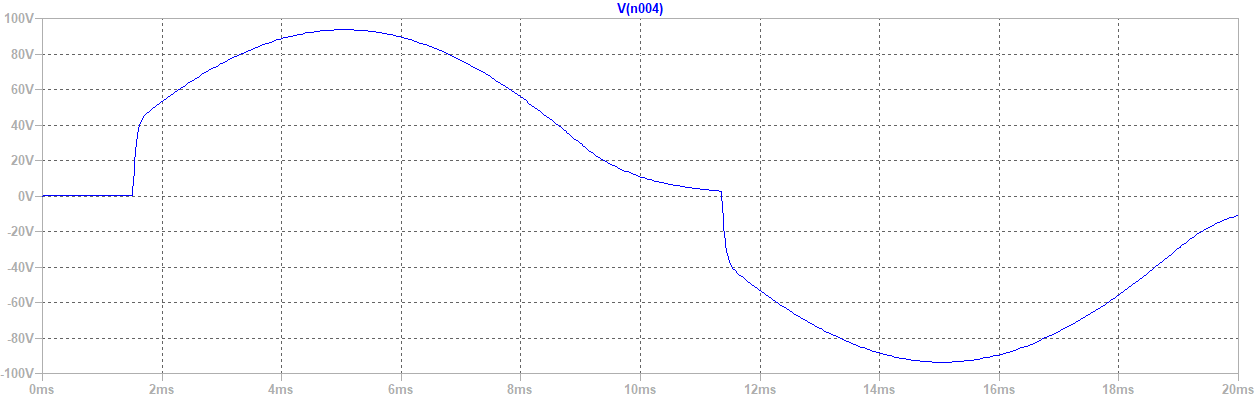
\includegraphics[scale=0.45]{R2-10k_C10u.png}
        \captionsetup{skip=0pt}
        \caption{Активно-емкостная нагрузка, $R=10\cdot10^3$ Ом, $C=10$ мкФ}
        \label{fig:R2-10k_C10u}
    \end{figure}
    \begin{figure}[H]
        \centering
        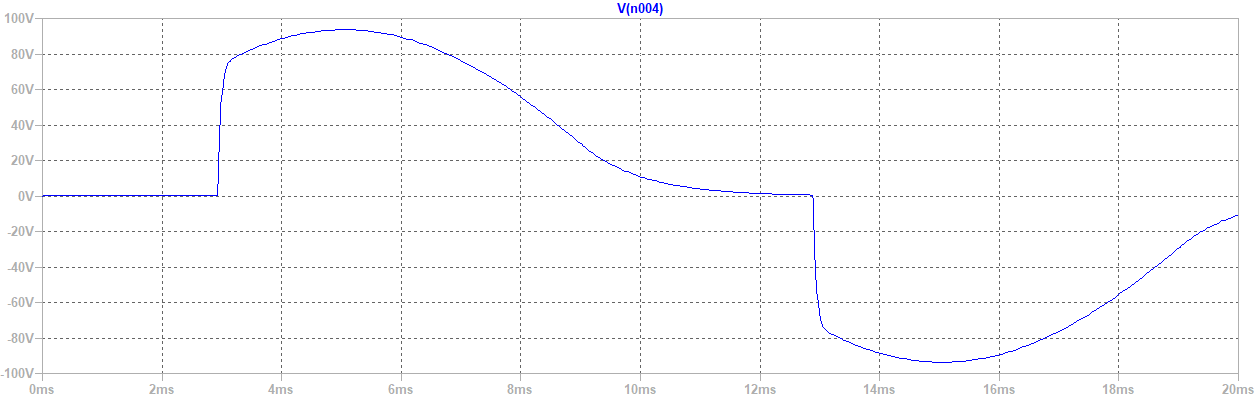
\includegraphics[scale=0.45]{R2-60k_C10u.png}
        \captionsetup{skip=0pt}
        \caption{Активно-емкостная нагрузка, $R=60\cdot10^3$ Ом, $C=10$ мкФ}
        \label{fig:R2-60k_C10u}
    \end{figure}
    \begin{figure}[H]
        \centering
        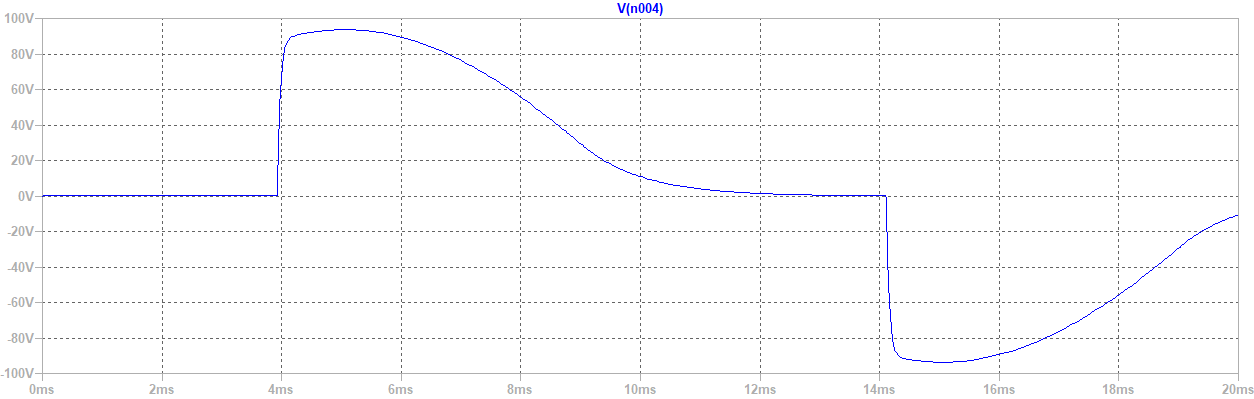
\includegraphics[scale=0.45]{R2-110k_C10u.png}
        \captionsetup{skip=0pt}
        \caption{Активно-емкостная нагрузка, $R=110\cdot10^3$ Ом, $C=10$ мкФ}
        \label{fig:R2-110k_C10u}
    \end{figure}
    \begin{figure}[H]
        \centering
        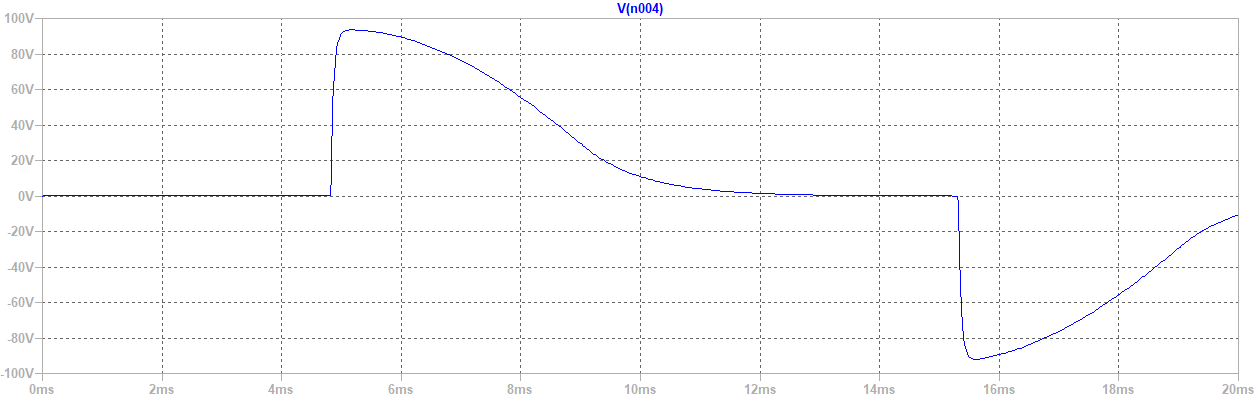
\includegraphics[scale=0.45]{R2-160k_C10u.png}
        \captionsetup{skip=0pt}
        \caption{Активно-емкостная нагрузка, $R=160\cdot10^3$ Ом, $C=10$ мкФ}
        \label{fig:R2-160k_C10u}
    \end{figure}
    \begin{figure}[H]
        \centering
        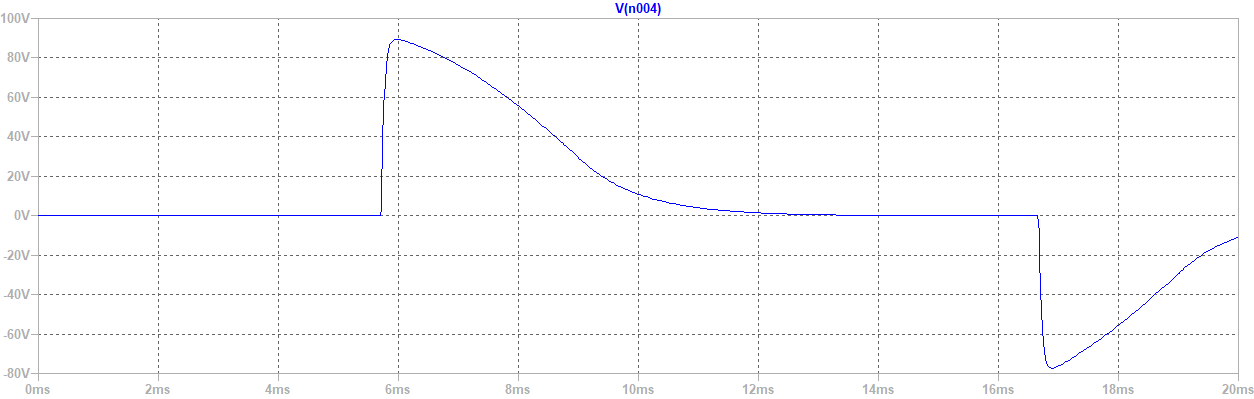
\includegraphics[scale=0.45]{R2-210k_C10u.png}
        \captionsetup{skip=0pt}
        \caption{Активно-емкостная нагрузка, $R=210\cdot10^3$ Ом, $C=10$ мкФ}
        \label{fig:R2-210k_C10u}
    \end{figure}
    \begin{figure}[H]
        \centering
        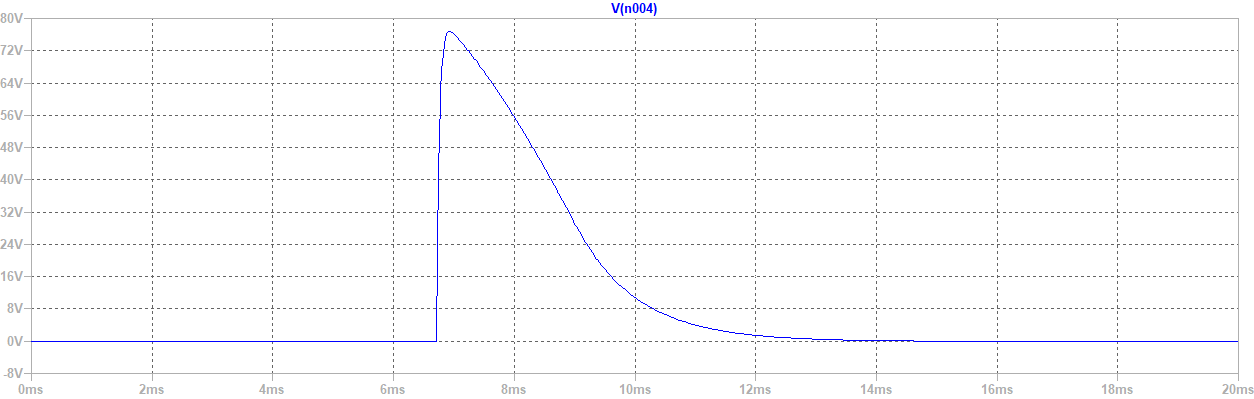
\includegraphics[scale=0.45]{R2-260k_C10u.png}
        \captionsetup{skip=0pt}
        \caption{Активно-емкостная нагрузка, $R=260\cdot10^3$ Ом, $C=10$ мкФ}
        \label{fig:R2-260k_C10u}
    \end{figure}
    \begin{figure}[H]
        \centering
        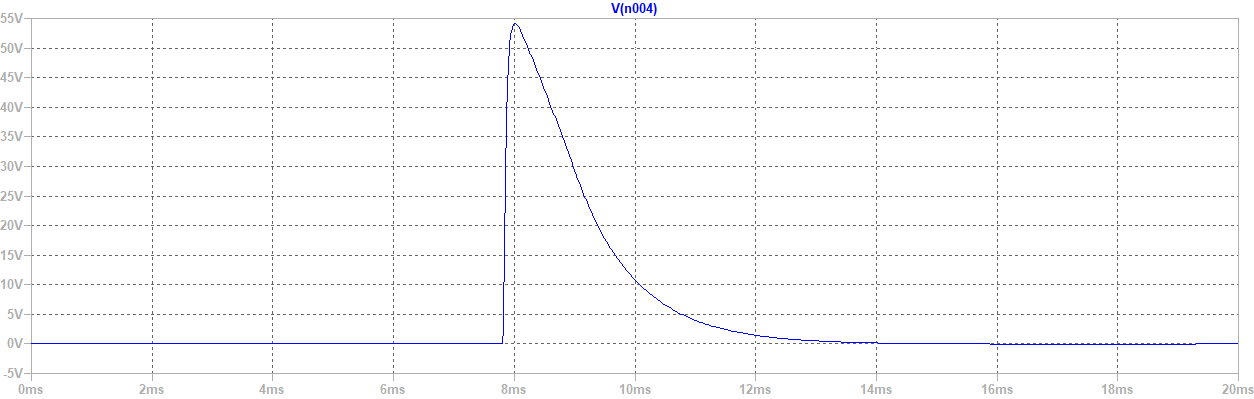
\includegraphics[scale=0.45]{R2-300k_C10u.png}
        \captionsetup{skip=0pt}
        \caption{Активно-емкостная нагрузка, $R=300\cdot10^3$ Ом, $C=10$ мкФ}
        \label{fig:R2-300k_C10u}
    \end{figure}


    \section{Вывод}
    В данной лабораторной работе были найдены регулировочные характеристики
    выпрямителя и регулятора напряжения. Были построены и смоделированы схемы,
    представлены результаты работы выпрямителя и регулятора напряжения в виде осцилограмм
    при различных типах нагрузки.


\end{document}